\setchapterpreamble[u]{\margintoc}
\chapter{Generation of multispectral point clouds}
\labch{multispectral_pc}
\label{sec:multispectral_pc}

\section*{About this chapter}

In this chapter, an efficient solution for the fusion of 1) visible, 2) thermographic and 3) multispectral information acquired by \acrshort{uas}s is proposed. Accordingly, the methodology proposed for image fusion in Chapter \ref{sec:image_fusion} is made effective while also being extended to 3D. Furthermore, the proposed work is developed using massively parallel algorithms, supported by \acrshort{gpu}s and multi-core \acrshort{cpu}s. Commercial software is used as a baseline for evaluating the efficiency of our framework. Besides parallel processing, this work is also intended for maximizing the size of point clouds by projecting images with lower resolution into 3D point clouds. The overall procedure is depicted in Figure \ref{fig:multi_thermal_overview}. It extends the procedure presented in Chapter \ref{sec:thermal_pc} by translating the projection to the \acrshort{gpu} and optimizing the processing with sorting techniques.

Hence, the main contributions presented in this chapter are 1) the fusion of multiple imagery datasets from \acrshort{uas}s and 2) the generation of larger point clouds than current commercial software with 3) lower response time. The accurate colour aggregation in 3D points is ensured by taking into account the occlusion of foreground surfaces. Accordingly, the proposed solution reconstructs much more dense point clouds than notable commercial software (286\% on average), e.g., Pix4Dmapper and Agisoft Metashape, in much less time (-70\% on average). 

\section{On the generation of point clouds augmented with multiple data sources}

Remote sensing research concerns multiple acquisition devices and multispectral data obtained in different wavelength ranges. These are frequently visible, infrared and multispectral imagery, either collapsed into a few or hundreds of bands (hyperspectral). Thus, the main challenge of multiple sensing systems is to fuse all this information into a sole data model with multiple layers. Fusion methodologies have been long investigated to build multi-layer models that allow subsequent analyses to focus only on the data. From these models, Machine Learning \cite{padua_vineyard_2022} and Deep Learning \cite{jia_survey_2021, hu_hyperspectral_2022} represent a widespread field to extract further information. Among other factors, the raising interest in 3D models is possible due to the use of \acrshort{uas} in \acrshort{rs}. In contrast to satellite imagery, \acrshort{uas}s provide a cost-efficient solution with higher spatial and temporal resolution \cite{singh_bibliometric_2022}. Nevertheless, vehicles and devices which are less prohibitive also lead to images with more defects and errors, either motivated by \acrshort{uas} instability \cite{akhoundi_khezrabad_new_2022} or the optical mechanism \cite{mohamad_screening_2021}. 
%Besides this, the reduced flight altitude requires wide-angle lenses that lead to geometric distortions. Though some of these errors can be corrected, the number of steps for data fusion increases and so does the overall complexity. 

The main drawback of 3D point clouds with hundreds of millions of points is to process them with commodity hardware. However, they are required to provide in-depth analyses and valuable renderings \cite{schutz_rendering_2021}. As a result, the reconstruction and processing of large point clouds are computationally demanding tasks that require massively parallel algorithms and modern \acrshort{gpu}s with increased capacity to operate many parallel threads. Therefore, solutions for fusing \acrshort{rs} data are not solely aimed at providing accurate results, but also at efficiently generating them. The baseline for the reconstruction of 3D point clouds can be established using commercial software, with most of them taking advantage of \acrshort{gpu}s to speed up the reconstruction \cite{jiang_efficient_2020}. Hence, their processing time is related both to the degree of parallelism as well as the size of input data. Accordingly, large point clouds are expected to worsen the performance, though they provide valuable data for mesh-like renderings and neighbourhood-derived processing (e.g., the estimation of normal vectors).   

\begin{figure*}[ht]
    \centering
    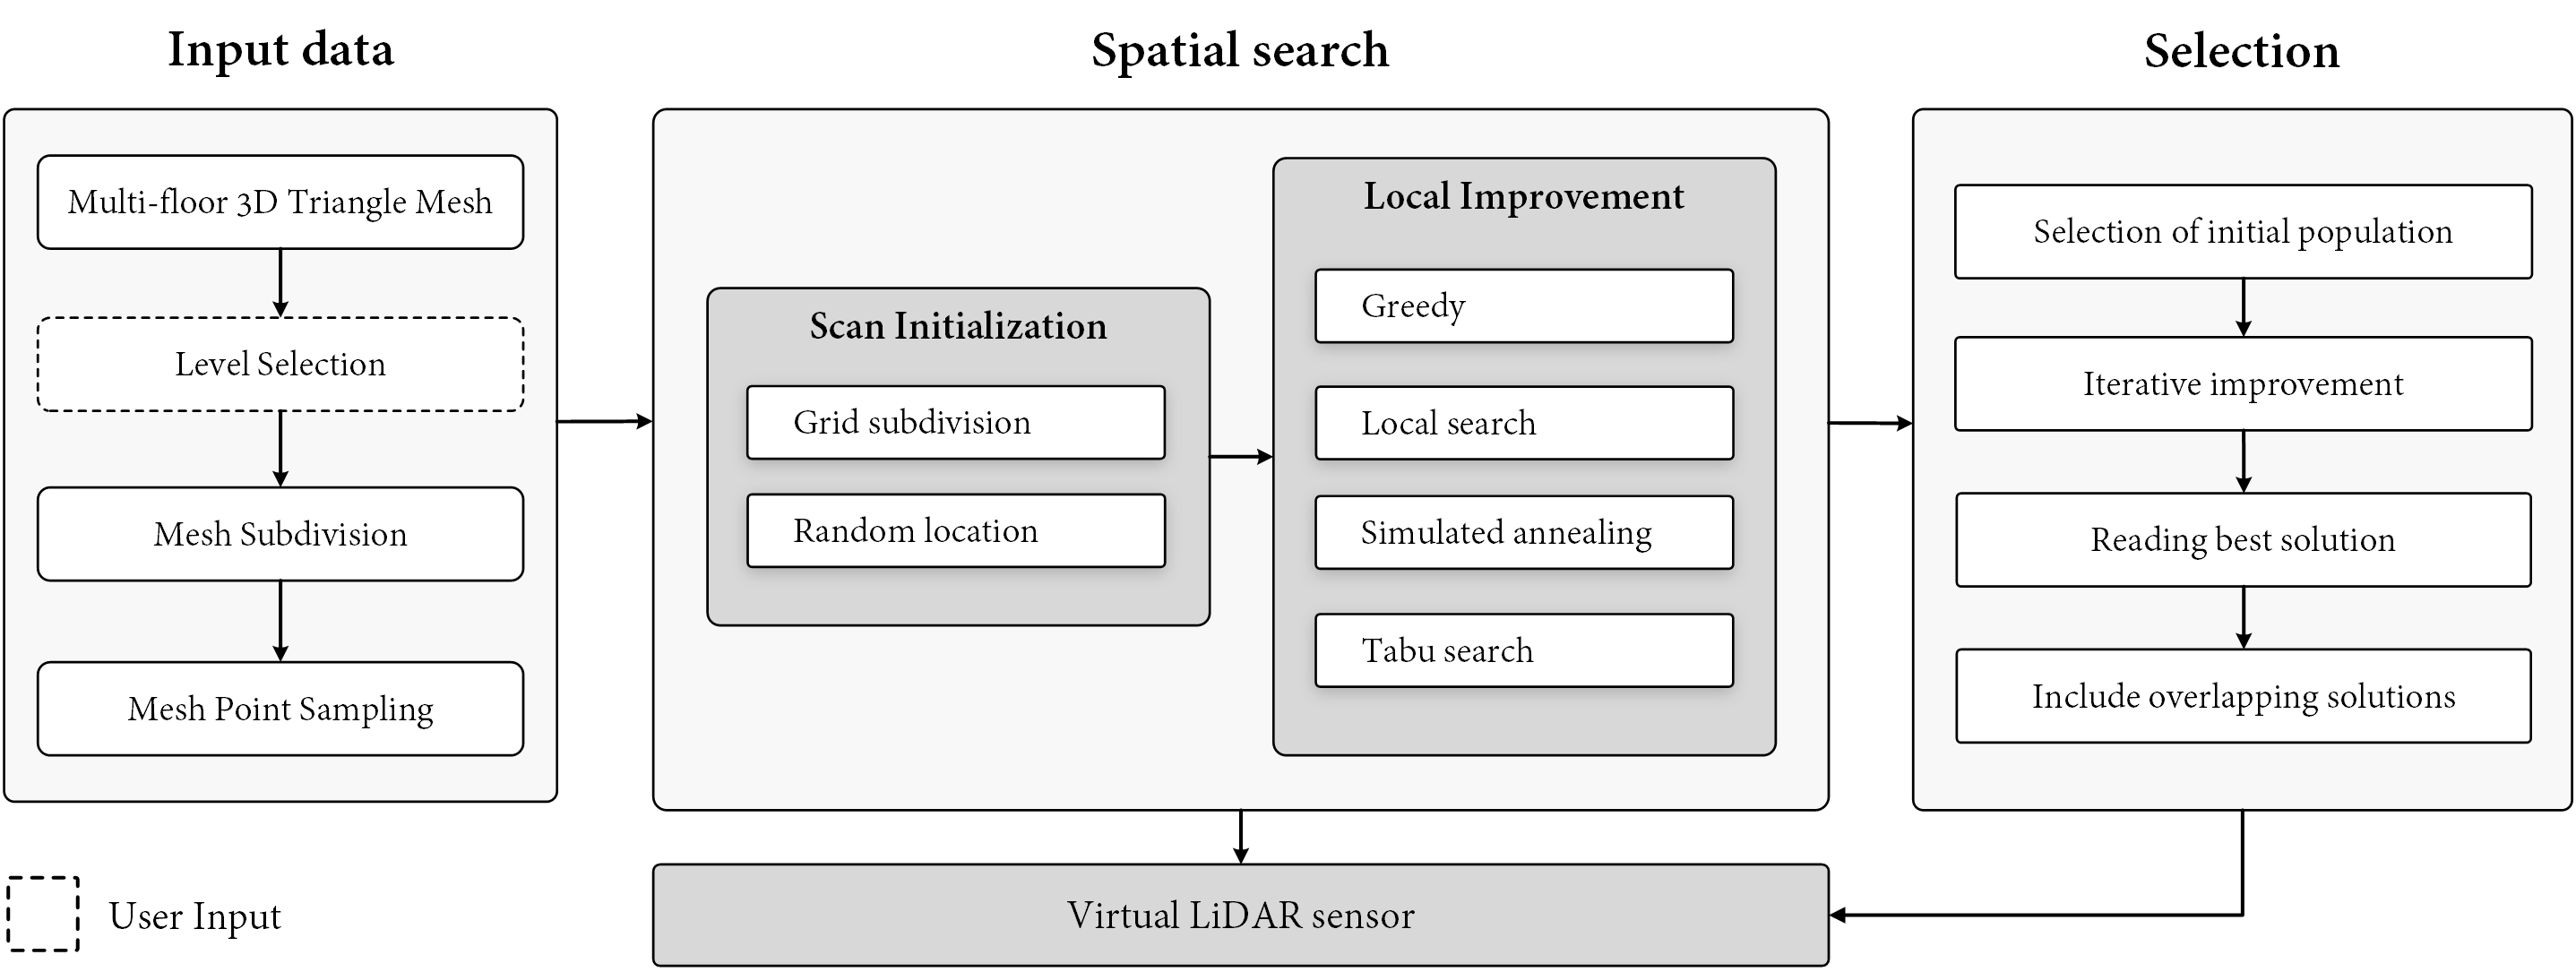
\includegraphics[width=.95\linewidth]{figs/multi_thermal_projection/overview.png}
    \caption{Overall procedure of the proposed method. First, the visible point cloud is reconstructed. Then, alternative data sources are projected into the previous point cloud. Finally, point clouds are aligned through the estimation of rigid transformations. The reconstruction of alternative point clouds is compared against popular commercial solutions. }
	\label{fig:multi_thermal_overview}
\end{figure*}

%-------------------------------------------------------------------------
\section{Correction and fusion of image datasets}

Images acquired either by thermographic or multispectral devices followed distinct distortion models, as previously explained. \acrshort{rgb} and multispectral imagery present fisheye distortion due to their lower focal length, though it is especially visible in multispectral images. Thermographic lenses have a larger focal length, resulting in a pincushion distortion effect. However, distortion correction can be parameterized by five coefficients (radial and tangential distortion coefficients: $k_1, k_2, p_1, p_2, k_3$) in both cases, along with the camera matrix, $K$. Hence, the correction of every dataset is performed regardless of the camera source. An exception to this is given by multispectral images, which define their own distortion model with four distortion coefficients arranged in a 3th-degree equation. Note that distortion coefficients are not frequently read from image metadata; instead, the bundle adjustment phase of \acrshort{sfm} is used to estimate these coefficients. 

According to the surveying devices, two different pipelines are here established. The first pairs visible images with thermographic data by determining the image's id and the corresponding co-acquired thermal image. Similarly to the described pipeline, multispectral images are linked to the source \acrshort{rgb} image. However, the latter image-matching is performed hierarchically, with the Green layer being the master one. Hence, properties of other layers are calculated according to this, including the matrices for fusing images. The result of this section is a composite matrix for every \acrshort{rgb} image, either relating it to a thermal or multispectral image. These are not related to more than one data source as they cannot be considered to be triggered synchronously. At this point, point clouds can be fed with additional information since their projection matrix to the \acrshort{rgb} image plane is known. 

%-------------------------------------------------------------------------
\section{Projection in 3D point clouds}

The following step is to project 3D points into their original data source. As occurs with photogrammetric pipelines, the \acrshort{rgb} point cloud is first generated since it represents the most accurate and dense 3D result. This model can be enhanced by including additional spectral information at every point. Otherwise, a low-density version of the \acrshort{rgb} point cloud would be generated from another data source. Hence, this work reuses the starting \acrshort{rgb} point cloud, whose viewpoints are calibrated during \acrshort{sfm}. Each viewpoint $c$ is associated with a projection matrix $P_c$ that allows mapping 3D points into individual \acrshort{rgb} image planes. From here, the previously computed inverse homography matrices allow translating \acrshort{rgb} coordinates into a different Cartesian coordinate system. Note that the projection of a 3D point for a viewpoint is not always within the image boundaries; indeed, only a few points will be mapped to each image. The main shortcoming is that some points will not be successfully mapped to any image, mainly those located at the boundaries. As a result, augmented point clouds have different dimensions than the baseline due to the smaller focal length of the rest of the devices in comparison with the \acrshort{rgb} sensor. Still, the resolution is preserved in terms of points per \si{\meter\squared}.

%-------------------------------------------------------------------------
\section{Occlusion}

The main drawback of the previously described projection is that spectral data from images could be projected into 3D points that were not visible from a viewpoint. Hence, this could lead to point clouds with incorrect radiometric data for additional layers. In this chapter, occlusion is handled using \textit{z}-buffers to capture the scene depth as grayscale values. Due to the aim of this work, \textit{z}-buffers also store the index of the nearest point projected at each pixel. In this manner, points that are more distant from the viewpoint than the point stored at the projected pixel are discarded.  From a $\infty$-filled image, points close to the viewpoint are projected to determine the minimum depth at each pixel, thus generating a \textit{z}-buffer similar to the output of depth sensors. However, \textit{z}-buffers with low resolution also lead to point clouds of lower density, as those generated by commercial software. To avoid this, the dimensionality of \textit{z}-buffers is upscaled by a factor $s$ to be determined in order to balance memory usage and the point cloud's density.

This task was solved using three different approaches. First, it was solved using \acrshort{opengl}'s built-in \textit{z}-buffers, then, these were constructed from scratch using \acrshort{opengl}'s compute shaders, and finally, a similar pipeline to \acrshort{opengl}'s compute shaders was followed using \acrshort{cuda}.

\newcommand{\Points}{\textrm{P}\textsubscript{\acrshort{gpu}}}
\newcommand{\Viewpoints}{\textrm{V}\textsubscript{\acrshort{cpu}}}
\newcommand{\Space}{\hspace{1mm}}
\newcommand{\Zbuffer}{z\textrm{-buffer}\textsubscript{GPU}}
\newcommand{\ZbufferCPU}{z\textrm{-buffer}\textsubscript{CPU}}
\newcommand{\Indices}{\textrm{indices}\textsubscript{\acrshort{gpu}}}
\newcommand{\Codes}{\textrm{codes}\textsubscript{\acrshort{gpu}}}
\newcommand{\PCCardinality}{|\Points|}
\newcommand{\LeftPoints}{\textrm{n}_\textsubscript{left}}
\newcommand{\CurrentPoints}{\textrm{n}_\textsubscript{current}}
\newcommand{\MaxPoints}{\textrm{n}_\textsubscript{max}}
\newcommand{\NumGroups}{\textrm{n}_\textsubscript{groups}}
\newcommand{\Pointa}{\textrm{p}\textsubscript{3D}}
\newcommand{\Pointb}{\textrm{p}\textsubscript{2D}}

\subsection{\acrshort{opengl}'s rendering}

% \begin{marginfigure}[.cm]
%     \caption{\acrshort{opengl} stages involved in rendering a point cloud.}
%     \label{fig:occlusion_opengl_zbuffer_core}
%     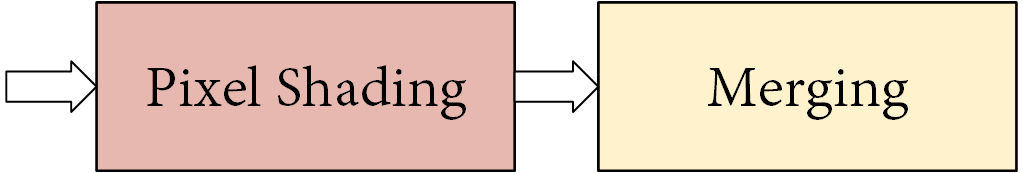
\includegraphics[width=\linewidth]{figs/multi_thermal_projection/occlusion_opengl_core.png}
% \end{marginfigure}
Constructing \textit{z}-buffers is straightforwardly solved with \acrshort{opengl} as it already addresses the occlusion in the rendering pipeline. More specifically, it is the merging phase at the end of the traditional rasterization pipeline that is in charge of determining which primitive is visible at each pixel \cite{akenine-moller_real-time_2018}. However, the desired outcome of the visibility test is a buffer with the indices of points which are visible from a camera pose. The workflow of this approach is shown in Figure \ref{fig:occlusion_opengl_zbuffer}.

\begin{marginfigure}[.2cm]
    \centering
    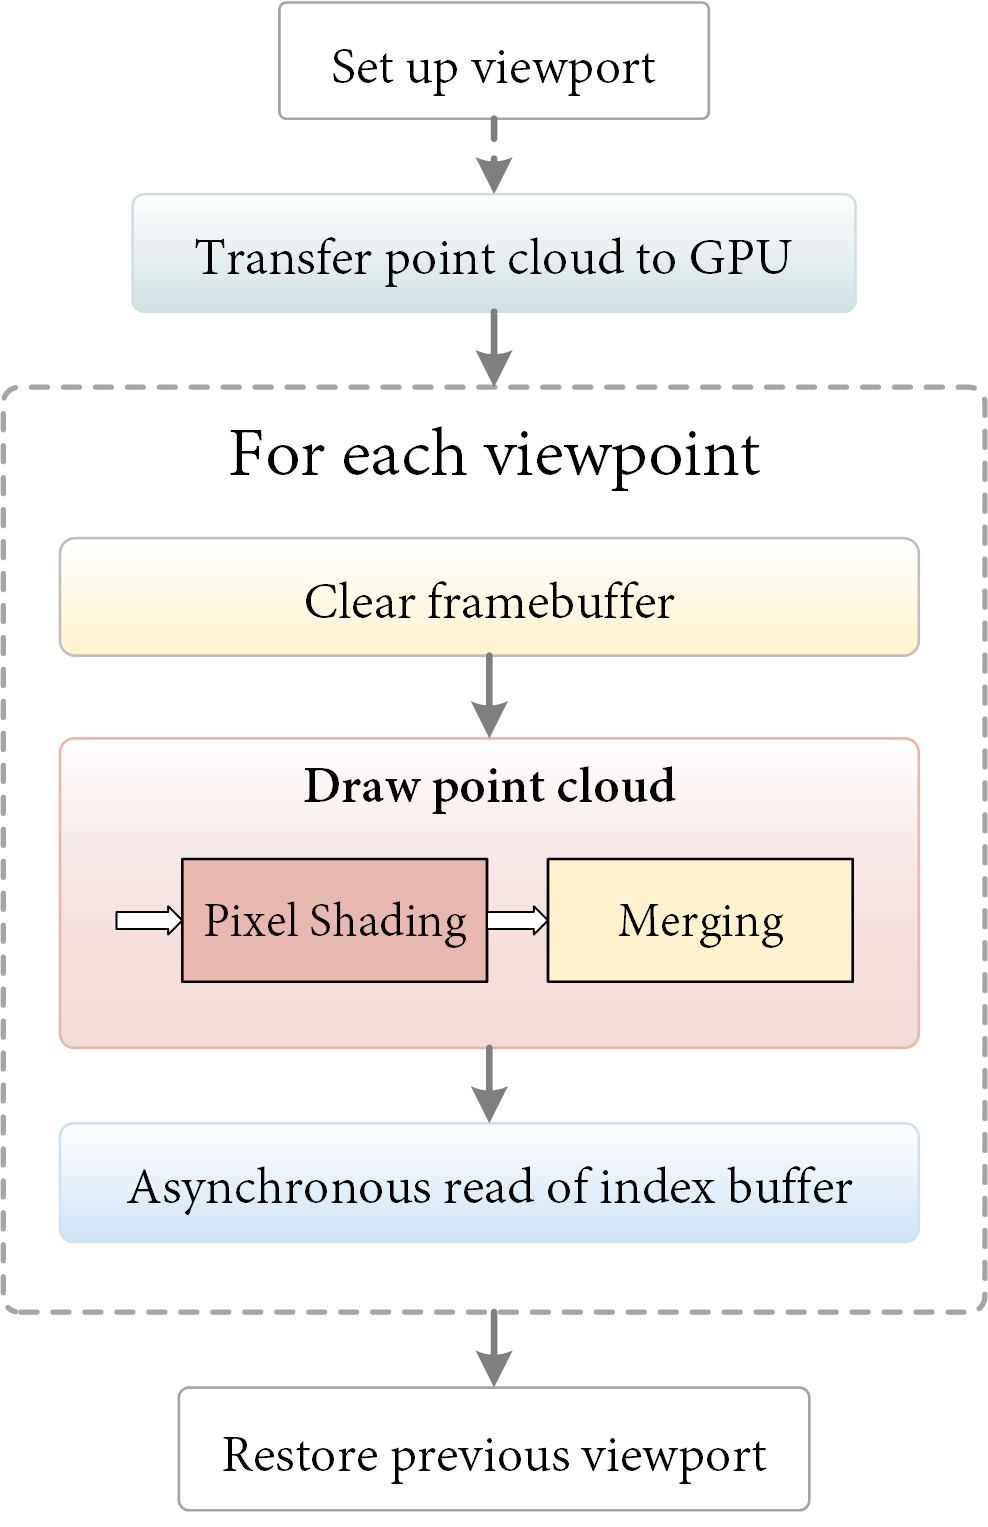
\includegraphics[width=\linewidth]{figs/multi_thermal_projection/occlusion_opengl.png}
    \caption{Workflow of the rendering-based methodology for a single batch of 3D points.}
    \label{fig:occlusion_opengl_zbuffer}
\end{marginfigure}
Points are transferred to the \acrshort{gpu} as \verb|vec4| values (i.e., four floating-point numbers) to fit the data alignment rules of subsequent sections. Also, a framebuffer comprising two textures of the same size is required; the first one collects point indices, whereas the second is a conventional \textit{z}-buffer. Clearing the framebuffer involves emptying the depth buffer and assigning a large value ($\infty$) to the index texture. Then, the whole point cloud is projected over the framebuffer to retrieve the nearest point visible at each pixel. Finally, the first texture is transferred to the \acrshort{cpu} via asynchronous reading (\verb|glReadPixels|). In contrast to the limited \acrshort{gpu} memory, \acrshort{cpu} storage is large enough to store a buffer of size $\abs{V} \cdot x \cdot y$, provided that $V$ is the image dataset, where each image has a resolution of $x, y$.

However, large point clouds may not fit in a single \acrshort{gpu} buffer. An alternative workflow is depicted in Figure \ref{fig:occlusion_opengl_zbuffer_multiple_batches}, with the maximum number of points depending on the maximum storage capacity. By default, the point cloud order is unknown and therefore iterations during this process are not disjoint. Consequently, the asynchronous reading involves reading the content of both depth and index buffers, which are then transferred to the \acrshort{gpu} for the next batch of points, instead of being reset. Transferring the downloaded \textit{z}-buffer content to the \acrshort{gpu} requires another rendering stage whose core is the built-in attribute \verb|gl_FragDepth| in the vertex shader. Also note that the framebuffer is not reset on each iteration, but only for the first batch of points. Another approach is to compute the results for each viewpoint in a single iteration, though it implies a huge increase in data transfers from \acrshort{cpu} to \acrshort{gpu}. The latter requires transferring every point cloud batch once per viewpoint ($\abs{V} \cdot n_{b}$), instead of $n_{b}$, with $n_{b}$ being the number of point cloud subdivisions.

\begin{figure}[htb]
    \centering
    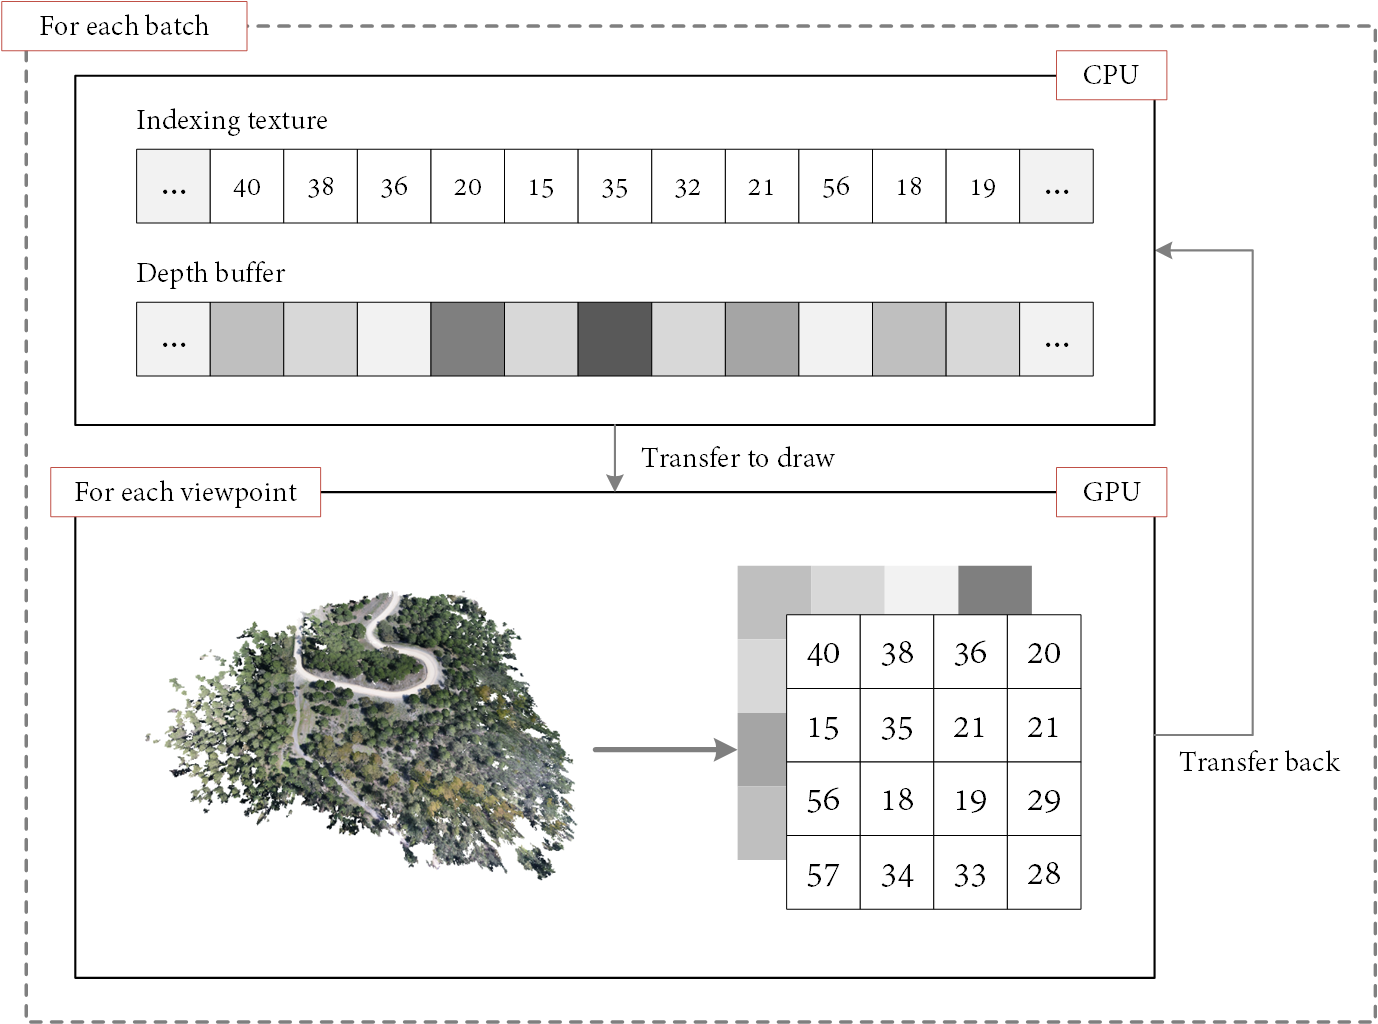
\includegraphics[width=.9\linewidth]{figs/multi_thermal_projection/multiple_batches_opengl_gpu.png}
    \caption{Overview of the rendering-based algorithm for multiple point cloud subdivisions.}
    \label{fig:occlusion_opengl_zbuffer_multiple_batches}
\end{figure}

\subsection{Compute shaders}

Compute shaders are general-purpose shaders for \acrshort{gpgpu}, and therefore, they can be applied to tasks not related to rendering. Unlike \acrshort{opengl}'s rendering pipeline, \textit{z}-buffers are not provided in this shader stage and thus must be implemented as a low-level mechanism supported by buffers known as Shader Storage Buffer Objects (\acrshort{ssbo}). Despite the lack of integrated \textit{z}-buffers, compute shaders provide a more efficient and flexible solution to read, write and perform trivial operations in buffers. Furthermore, it avoids some unnecessary stages from the rendering pipeline, including polygon rasterization and interpolations. 

\begin{marginfigure}[.cm]
    \caption{Compute shader steps involved in rendering a point cloud.}
    \label{fig:occlusion_compute_shader_zbuffer_core}
    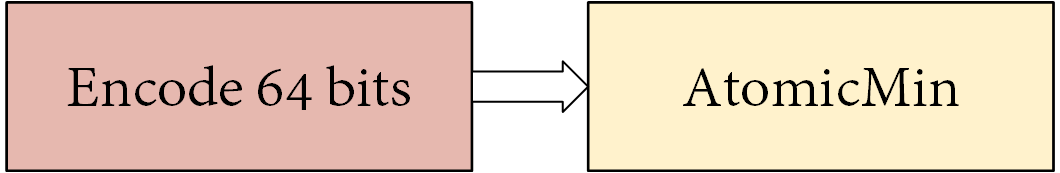
\includegraphics[width=\linewidth]{figs/multi_thermal_projection/occlusion_compute_shader_core.png}
\end{marginfigure}
Regarding memory allocation, \textit{z}-buffers are here modelled as integers of 64 bits (\verb|uint64_t|) using \acrshort{opengl}'s modern extensions, to be equally split between distance and index. Distance is not a numeric integer, $d \in \mathbb{R}$, though its low-level representation can be interpreted as an integer using \verb|floatBitsToUint|. For a viewpoint, $\textit{xyz}_c$, and a 3D point ($\textit{xyz}_p$) with index $i_p$, the Euclidean distance is computed, transformed into an integer and concatenated to $i_p$ (Equation \ref{eq:concatenation}). With this representation, fewer and greater comparisons work as usual. Thus, these operators can be applied to build a \textit{z}-buffer by selecting the minimum distance while also carrying the point index. To this end, the atomic $\min$ operator (\verb|atomicMin|) is used.
\begin{equation}
    \label{eq:concatenation}
    z_{k, l} \gets \lVert\textit{xyz}_p - \textit{xyz}_c\rVert ^\frown x_p
\end{equation}

The procedure to project the point cloud into $z$-buffers is following described in Algorithm \ref{alg:gpu_single_batch} if it fits in the \acrshort{gpu}'s \acrshort{vram} and the maximum size of \acrshort{opengl}'s buffers (see Figure \ref{fig:occlusion_compute_shader_zbuffer}). Otherwise, Algorithm \ref{alg:gpu_multiple_batch} is followed. Note that the second scenario omits the smaller procedures shown in Algorithm \ref{alg:gpu_single_batch}. Because data transfers of $z$-buffers in \acrshort{cpu} $\leftrightarrow$ \acrshort{gpu} are notably smaller, point batches are iterated in the outer $\textit{for}$ and thus are only transferred once. Instead, each viewpoint's $z$-buffer is transferred once per point batch. Once all the points have been projected into every $z$-buffer, the indices indicating which points are visible are read, as proposed in Algorithm \ref{alg:gpu_single_batch}.
\begin{marginfigure}[.3cm]
    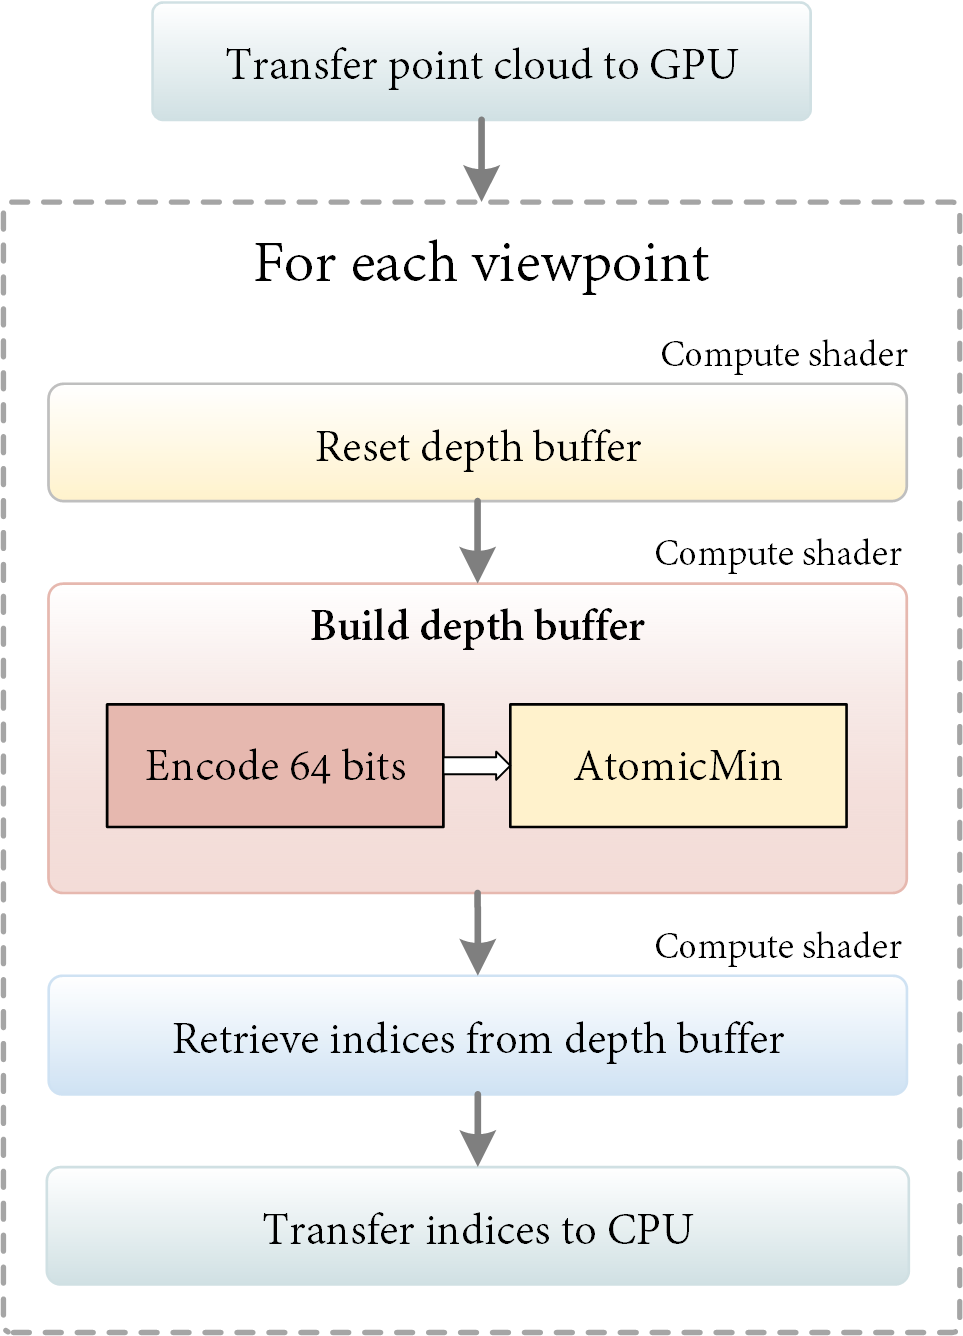
\includegraphics[width=\linewidth]{figs/multi_thermal_projection/occlusion_compute_shader.png}
    \caption{Overview of methodology based on compute shaders for a single batch of 3D points.}
    \label{fig:occlusion_compute_shader_zbuffer}
\end{marginfigure}

\begin{algorithm}
      \small
      \begin{algorithmic}[1]
        \State \textbf{Input} 3D \acrshort{rgb} points: \Points %\;
    	\State \textbf{Input} Viewpoints with dimensionality $x \cdot y$: $\Viewpoints$ %\;
        \State \textbf{Variable} \textrm{thread}\textsubscript{id} in the \acrshort{gpu}: id %\;
        \State \textbf{Output} \acrshort{rgb} point cloud with augmented thermal or multispectral data %\;        
        % \State Points are notated as \Points \hspace{1mm} and $\Viewpoints$ are camera viewpoints whose images have dimensionality $x \cdot y$. The term id refers to \textrm{thread}\textsubscript{id} in the \acrshort{gpu}. %\;
        \State Build $\Zbuffer \gets \textrm{uint64}(x \cdot y)$ and $\Indices \gets \textrm{uint}(x \cdot y)$ %\;
        \If{Sort \Points}
            \State $\Points \gets \textrm{sortPoints}(\Points)$   \Comment(Algorithm \ref{alg:sorting}) %\;
        \EndIf
        \Procedure{Build \textit{z}-buffers}{}
            \For {$v \Space \textrm{in} \Space \Viewpoints$}
                \State $M \gets v\textsubscript{projection}$ %\;
                \Procedure{Reset \textit{z}-buffer in \acrshort{gpu}}{}
                    \State $\Zbuffer_{i} \gets \textrm{UINT64\textsubscript{MAX}} \Space \forall i \in \left[0, x \cdot y\right[$ %\;
                \EndProcedure
                \Procedure{Fill \textit{z}-buffer in \acrshort{gpu}}{$M$, $v_p$}
                    \State $\Pointa \gets \Points\left[\textrm{id}\right]$ %\;
                    \State $\Pointa \gets \left[M \cdot \left[\Pointa_x, \Pointa_y, \Pointa_z, 1\right]^T\right]_{xyz}^T$ %\;
                    \State $\Pointb \gets \left[\Pointa_x / \Pointa_z, \Pointa_y / \Pointa_z\right]^T$ %\;
                    \If{\Pointb \Space inside image}
                        \State $\textrm{dist} \gets \textrm{floatBitsToUint}(\textrm{length}(\Pointa - v_p))$ %\;
                        \State $\textrm{tag} \gets \textrm{p}\textsubscript{index} | \left(\textrm{dist} << 32\right)$ %\;
                        \State $\textrm{atomicMin}(\Zbuffer\left[\textrm{id}\right], \textrm{tag})$ %\;
                    \EndIf
                \EndProcedure
                \Procedure{Obtain indices from \textit{z}-buffer}{}
                    \State $\textrm{index}\left[\textrm{id}\right] \gets \Zbuffer\left[\textrm{id}\right] \& \textrm{UINT\textsubscript{MAX}}$ %\;
                \EndProcedure
                \State $\textrm{visible\_points} \gets \Indices$ %\;
                \State Obtain point cloud colours in $\textrm{visible\_points}$ %\;
            \EndFor
        \EndProcedure
        \caption{Simplest case for projecting points in \textit{z}-buffers, where all the points fit in the \acrshort{gpu}'s \acrshort{vram}.}
        \label{alg:gpu_single_batch}
      \end{algorithmic}
      \normalsize
\end{algorithm}

\begin{algorithm}
    \small
    \begin{algorithmic}[1]
        \State \textbf{Input} 3D \acrshort{rgb} points: \Points %\;
    	\State \textbf{Input} Viewpoints with dimensionality $x \cdot y$: $\Viewpoints$ %\;
    	\State \textbf{Input} Maximum number of points that can be allocated in the \acrshort{gpu}: $\MaxPoints$ %\;
        \State \textbf{Variable} \textrm{thread}\textsubscript{id} in the \acrshort{gpu}: id %\;
        \State \textbf{Output} \acrshort{rgb} point cloud with augmented thermal or multispectral data %\;  
        % \State $\Points$ refers to points, $\Viewpoints$ are camera viewpoints whose images have dimensionality $x \cdot y$ and $\MaxPoints$ is the maximum number of points that can be allocated in the \acrshort{gpu}. %\;
        \State Build $\Zbuffer\acrshort{cpu} \gets \textrm{uint64}(x \cdot y \cdot |\Viewpoints|)$ %\;
        \State $\Zbuffer\acrshort{cpu}_{i} \gets \textrm{UINT64\textsubscript{MAX}} \Space \forall i \in \left[0, x \cdot y \cdot |\Viewpoints|\right[$ %\;
        \State Build $\Zbuffer \gets \textrm{uint64}(x \cdot y)$ and $\Indices \gets \textrm{uint}(x \cdot y)$ %\;
        \State $\LeftPoints \gets \PCCardinality$ %\;
        \If{Sort \Points}
            \State $\Points \gets \textrm{sortPoints}(\Points)$   \Comment(Algorithm \ref{alg:sorting}) %\;
        \EndIf
        \While{$\LeftPoints > 0$}
            \State $\CurrentPoints \gets \textrm{min}(\LeftPoints, \MaxPoints)$ %\;
            \State Transfer point batch to \acrshort{gpu} %\;
            \For {$v \Space \textrm{in} \Space \Viewpoints$}
                \State Transfer to \acrshort{gpu} part of $\Zbuffer\acrshort{cpu}$ from $v$ %\;
                \State Complete $\Zbuffer$ with current point batch %\;
                \State Read $\Zbuffer$ into the pointer of $\Zbuffer\acrshort{cpu}$ %\;
            \EndFor
            \State Update $\LeftPoints$ %\;
        \EndWhile
        \For {$v \Space \textrm{in} \Space \Viewpoints$}
            \State Transfer to \acrshort{gpu} part of $\Zbuffer\acrshort{cpu}$ from $v$ %\;
            \State Split indices from \Zbuffer \hspace{1mm} into \Indices %\;
            \State $\textrm{visible\_points} \gets \Indices$ %\;
            \State Obtain point cloud colours in $\textrm{visible\_points}$ %\;
        \EndFor
        \caption{The point vector is split if it does not fit in the \acrshort{gpu}'s \acrshort{vram} during their projection in \textit{z}-buffers.}
        \label{alg:gpu_multiple_batch}
      \end{algorithmic}
      \normalsize
\end{algorithm}

\subsection{\acrshort{cuda}}

The \acrshort{cuda} kernel for computing the nearest 3D point for every pixel and viewpoint is analogous to the compute shader workflow. The main advantage of the \acrshort{cuda} implementation is that it enables overlapping the \acrshort{cpu} $\leftrightarrow$ \acrshort{gpu} transfers with the \acrshort{gpu} processing. The use of multiple \acrshort{cuda} streams exploits asynchronous transfer operations and kernel executions to achieve an efficient result. Hence, points from a batch are projected in the \acrshort{cuda} kernel while the next batch is being transferred to \acrshort{gpu}. Similarly, results are downloaded from the \acrshort{cpu} while a viewpoint is being processed by the current kernel.

% \vspace{3mm}

% \lstinputlisting[language=c++, caption={Overlapping execution of different data streams per point cloud batch.}, label=code:occlusioncuda]{code/cuda_occlusion.cpp}

%-------------------------------------------------------------------------
\section{Point cloud sorting}

\begin{marginfigure}[-1cm]
    \centering
    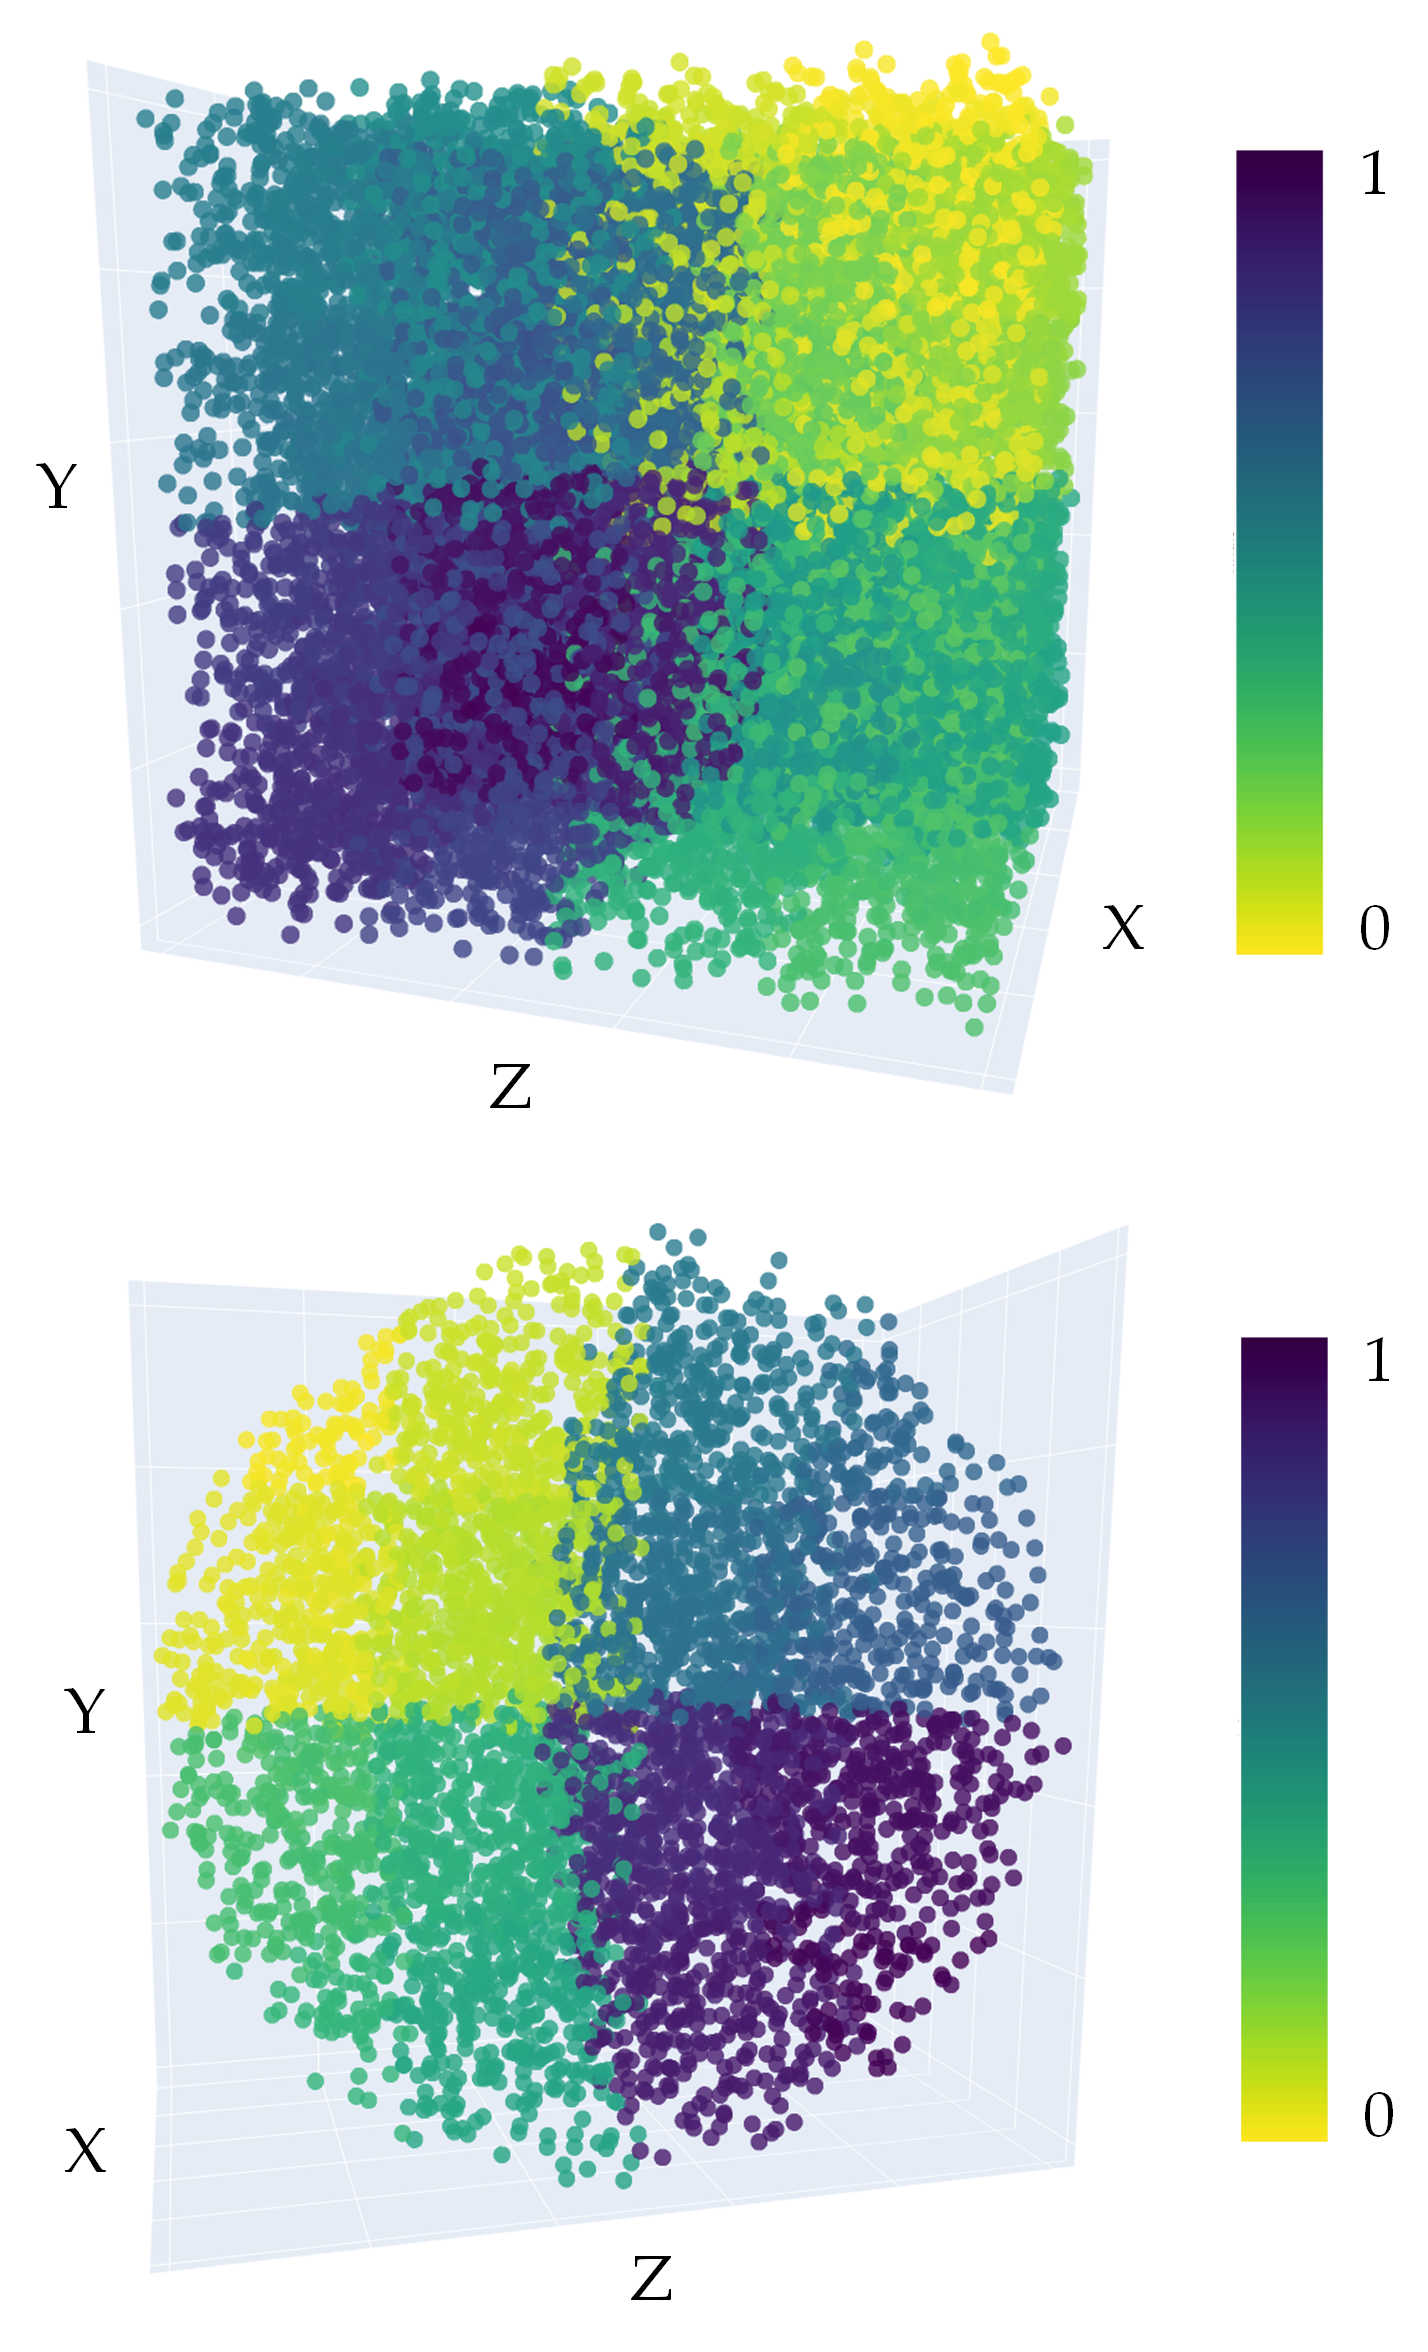
\includegraphics[width=\linewidth]{figs/multi_thermal_projection/point_cloud_morton.png}
    \caption{Colouring of two randomized point clouds in [0, 1] according to Morton encoding with 30 bits. }
	\label{fig:morton_point_cloud}
\end{marginfigure}
Point clouds generated by software present an unknown order regardless of their coordinates, \textit{xyz}. However, the outcome of previous projections is highly influenced by the sampled 3D volume; the points from a relatively small volume can be visible from a camera viewpoint while the others are discarded. Therefore, point clouds whose primitives have an unknown order also require unordered updates in memory buffers. On the other hand, organized updates are known to be more efficient due to faster memory writing. Although there is no such ordering in 3D space, there exist methods for the hierarchical clustering of geometry, such as the \textit{Z}-order curve depicted in Figure \ref{fig:morton_point_cloud}. The outcome is a 1D buffer where points which have close indices also happen to be in close spatial positions. 

For large point clouds, changing their order presents a significant delay even for the most efficient sorting algorithms. Therefore, \acrshort{gpgpu} programming allows sorting them in parallel to reduce the response time during the projection procedure. In this work, Radix sort is used and adapted to \acrshort{gpgpu} by splitting it into two different steps: 1) up-sweep (reduce) and 2) down-sweep \cite{nguyen_gpu_2007}. Following this approach, the buffer is sorted with a complexity of $\mathcal{O}(mn)$, with $m$ being the number of bits and $n$ being the number of points. Prior to sorting, \textit{xyz} coordinates are converted to values of 30 bits ($m$) that encode individual coordinates (10 bits for each one). These have been previously revised as Morton codes, though they can have a variable bit length.

Despite the enhancement derived from sorting, \acrshort{gpu}-based algorithms are handled on the \acrshort{gpu} through work groups. These are small groups of threads that are allowed to share data. Thus, the main drawback of globally sorting the point cloud buffer is that the workload is not uniformly shared among work groups. Instead, the ordered buffer can be shuffled according to the size of the workgroups. The algorithmic flow for the described sort configuration is shown in Algorithm \ref{alg:sorting}. First, points are sorted with Radix Sort following the Morton encoding. Otherwise, a random order is used. Then, the point buffer can be reordered according to groups of size n\textsubscript{shuffle}. The second stage is implemented as a multi-core \acrshort{cpu} algorithm rather than in the \acrshort{gpu} to avoid duplicating large point buffers with limited \acrshort{vram}.

\section{Alignment of heterogeneous data sources}

The image-matching procedure was performed over different data sources from the same devices, e.g., visible and thermal data. With this approach, images are known to be acquired with a similar timestamp, and thus \acrshort{ecc} converges in a reasonable time. However, \acrshort{rgb} point clouds can be reused for different data sources whether they are represented in the same local coordinate system. Despite georeferencing providing accurate positioning, point clouds from distinct data sources may not exactly overlap. Hence, point clouds can be further aligned by finding the rigid transformation matrix with a precision below a threshold (Figure \ref{fig:icp}). In this chapter, it is implemented using the \acrshort{icp} algorithm.

\begin{figure}[ht]
    \centering
    \includegraphics[width=\linewidth]{figs/multi_thermal_projection/ICP.png}
    \caption{\acrshort{icp} registration process: a) \acrshort{rgb} point cloud from the first dual device, b) \acrshort{rgb} point cloud from the second dual device, and c) both point clouds aligned by minimizing their distance, with $G$ referring to a global system.}
    \label{fig:icp}
\end{figure}

\begin{algorithm}
  \begin{algorithmic}[1]
    \small
    \State \textbf{Input} Point cloud: $\Points$ %\;
    \State \textbf{Input} Maximum number of points that can be allocated in the \acrshort{gpu}: $\MaxPoints$ %\;
    \State \textbf{Variable} \textrm{thread}\textsubscript{id} in the \acrshort{gpu}: id %\;
    \State \textbf{Output} Sorted point cloud %\;  
    \State $\LeftPoints \gets \PCCardinality$ %\;
    \State $\textrm{indices} \gets \textrm{uint}\left[\PCCardinality\right]$ %\;
    \While{$\LeftPoints > 0$}
        \State $\CurrentPoints \gets \textrm{min}(\LeftPoints, \MaxPoints)$ %\;
        \State Transfer the following $\CurrentPoints$ batch to \acrshort{gpu} %\;
        \Procedure{Sort in \acrshort{gpu}}{}
            \State $\Codes \gets \textrm{morton\acrshort{gpu}}(\Points)$ %\;  
            \State $\textrm{indices} \gets \textrm{RadixSort}(\Points, \Codes)$ %\;
            \Procedure{$\textrm{RadixSort}(\Points, \Codes)$}{}
                \For {$\textrm{bit} \gets 0 \to 30$} 
                    \State Apply bit mask $1 << \textrm{bit to} \Points$ %\;
                    \State Up-sweep phase of prefix scan %\;
                    \State Reset last position to zero %\;
                    \State Down-sweep phase of prefix scan %\;
                    \State Reorder \Points with new positions %\;
                \EndFor
            \EndProcedure
        \EndProcedure
        \Procedure{Sort in multi-core \acrshort{cpu}}{}
            \If{Shuffle}
                \State $\NumGroups \gets \lceil \CurrentPoints / \textrm{n}\textsubscript{shuffle} \rceil$ %\;
                \State rdn\textsubscript{group} $\gets \textrm{RandomVector}(\NumGroups, 0, 1)$ %\;
                \State iota\textsubscript{group} $\gets \bigl[0, 1, ..., \NumGroups-1 \bigr]$ %\;
                \State id\textsubscript{old}, id\textsubscript{new} $\gets$ Sort($\textrm{rdn\textsubscript{group}}, \textrm{iota}\textsubscript{group}$) %\;
                \For {group in $\left(\textrm{id}\textsubscript{old}, \textrm{id}\textsubscript{new} \right)$}
                    \State Move point batch from $\textrm{id}\textsubscript{old}$ to $\textrm{id}\textsubscript{new}$ %\;
                \EndFor
            \Else
                \State Reorder points with indices %\;
            \EndIf
        \EndProcedure
        \State Update \Points \Space and $\LeftPoints$ with $\CurrentPoints$ %\;
    \EndWhile
    \caption{Point cloud sorting.}
    \label{alg:sorting}
  \end{algorithmic}
  \normalsize
\end{algorithm}

\section{Results and discussion}

\begin{figure*}
    \centering
    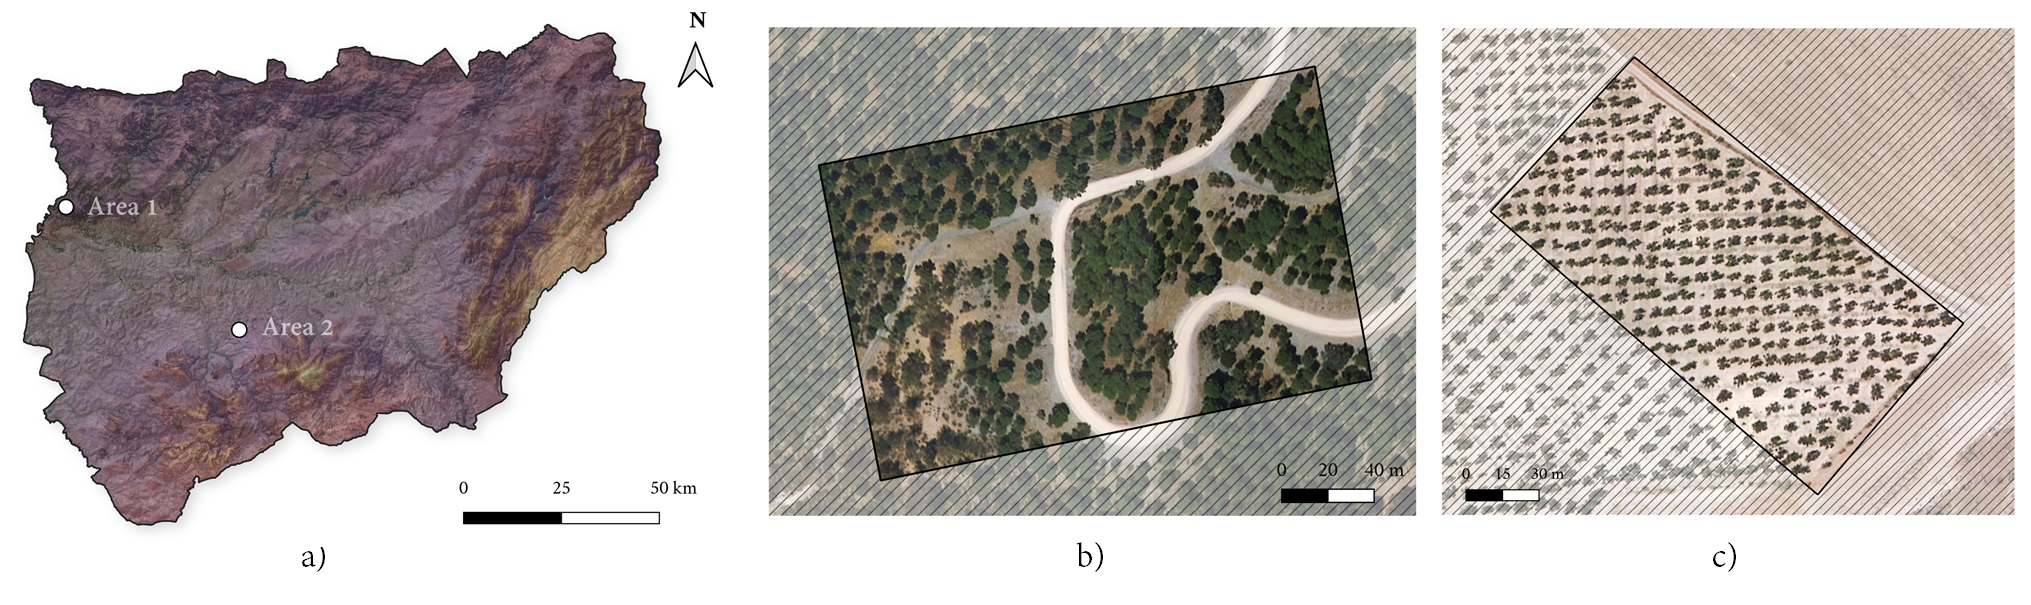
\includegraphics[width=.97\linewidth]{figs/multi_thermal_projection/study area.png}
    \caption{Overview of the surveyed region and areas. a) The region of Jaén, b) a forest and c) an olive grove. }
\label{fig:occlusion_study_area}
\end{figure*}

In this section, the proposed methodology is compared with other notable software solutions for building multispectral and thermal point clouds, such as Pix4Dmapper or Agisoft Metashape. The carried tests are focused on obtaining the response time and point cloud size, although some reconstructions from these solutions also present geometrical errors. The evaluation was performed on a PC with AMD Ryzen Threadripper 3970X 3.6 GHz, 256 GB RAM, two NVIDIA RTX A6000 \acrshort{gpu}s and Windows 10 \acrshort{os}. The proposed methodology was implemented in C++ using \acrshort{opengl}, and besides \acrshort{gpu} computing, \acrshort{cpu}-based methods were accelerated using the Open Multi-Processing (\acrshort{openmp}) framework.

The baseline \acrshort{rgb} point cloud consists of 115M (multispectral) and 97M (thermal) points for the first dataset, whereas the second dataset yields point clouds with a dimensionality of 126M and 96M points. To further stress this evaluation and achieve higher point density, a single depth buffer resolution has been used, $d\gets 10$. Regarding point cloud order, points are initially shuffled to show the benefits of spatial sorting. Apart from this, two different setups are here shown: 1) sorting with Morton codes and 2) sorting and shuffling in small groups. The experimental results are obtained by repeating every test four times and averaging the results. 

\begin{kaobox}[frametitle=\acrshort{opengl} and \acrshort{cuda} comparison]
This chapter comprises the last work of this dissertation, with compute shaders being the preferred solution. Other presented approaches use \acrshort{opengl}'s rendering pipeline as well as the \acrshort{cuda} framework to perform this very same operation. However, the latter comparison was performed in a work published in the \textbf{Proceedings of the 2021 Spanish Conference in Computer Graphics}. In this work, tests were performed on a PC with Intel Core i9-9900 3.1 GHz, 48 GB RAM, RTX 2080 Ti \acrshort{gpu} with 11 GB RAM (Turing architecture) and Windows 10 \acrshort{os}, using C++, \acrshort{cuda} and \acrshort{opengl}. The dataset was the first one explained (forestry area), although the input cloud had 271 million points which were observed from 1352 viewpoints. A simplified version of this comprises 66 million points and 180 viewpoints. 
\end{kaobox}

Regarding the configuration of commercial solutions, the steps of image alignment and reconstruction of a dense point cloud (i.e., densification) were performed with the highest quality. Since both of them are known to be able to use \acrshort{cuda}-enabled \acrshort{gpu}s, they were enabled to accelerate their pipeline on the \acrshort{gpu}. Furthermore, the latter is known to be accelerated with the multi-\acrshort{gpu} framework \acrshort{cuda} and therefore, was expected to perform better since two \acrshort{gpu}s were available.  

\subsection{Study area}

The proposed method has been evaluated over two different environments located in the region of Jaén, Spain. To show its effectiveness in multiple fields, data depicting 1) a forestry area and 2) an olive grove was processed. Hence, the results will prove that the fusion of information works well in scenarios with more significant features (2) and not recognizable features (1). Figure \ref{fig:occlusion_study_area} shows the location of both areas. The flight altitude was 454 \si{\meter} and 595 \si{\meter} above sea level, respectively. The forestry scene is composed of repetitive patterns from vegetation and human-made structures. The first area covers nearly 1.97 \si{\hectare}, whereas the second includes 2.44 \si{\hectare}.

\subsection{Image processing}

The image alignment stage is configured according to the \acrshort{ecc} parameters: 1) the number of iterations to converge and 2) the aimed precision. The first is set to 400 iterations to sufficiently cover the number of required iterations. The precision is set to the default value, $\epsilon \gets 1^{-3}$. Besides these parameters, the dimensionality of the compared images is also relevant since the lesser number of details also implies a faster convergence. However, images were not downscaled in this study to ensure that a fine-grained alignment is achieved. Finally, the hierarchical alignment of multispectral images is also studied by means of confusion matrices that show the correlation of pairs of bands. Accordingly, Figure \ref{fig:occlusion_confusion_matrices} justifies the hierarchy shown in Figure \ref{fig:ecc_hierarchy}. Note that \acrshort{nir} and \acrshort{reg} layers are reciprocally the most similar. However, \acrshort{reg} images are more similar to the root, Green, and thus \acrshort{nir} layers were aligned to \acrshort{reg} images.

\begin{figure*}[ht]
    \centering
    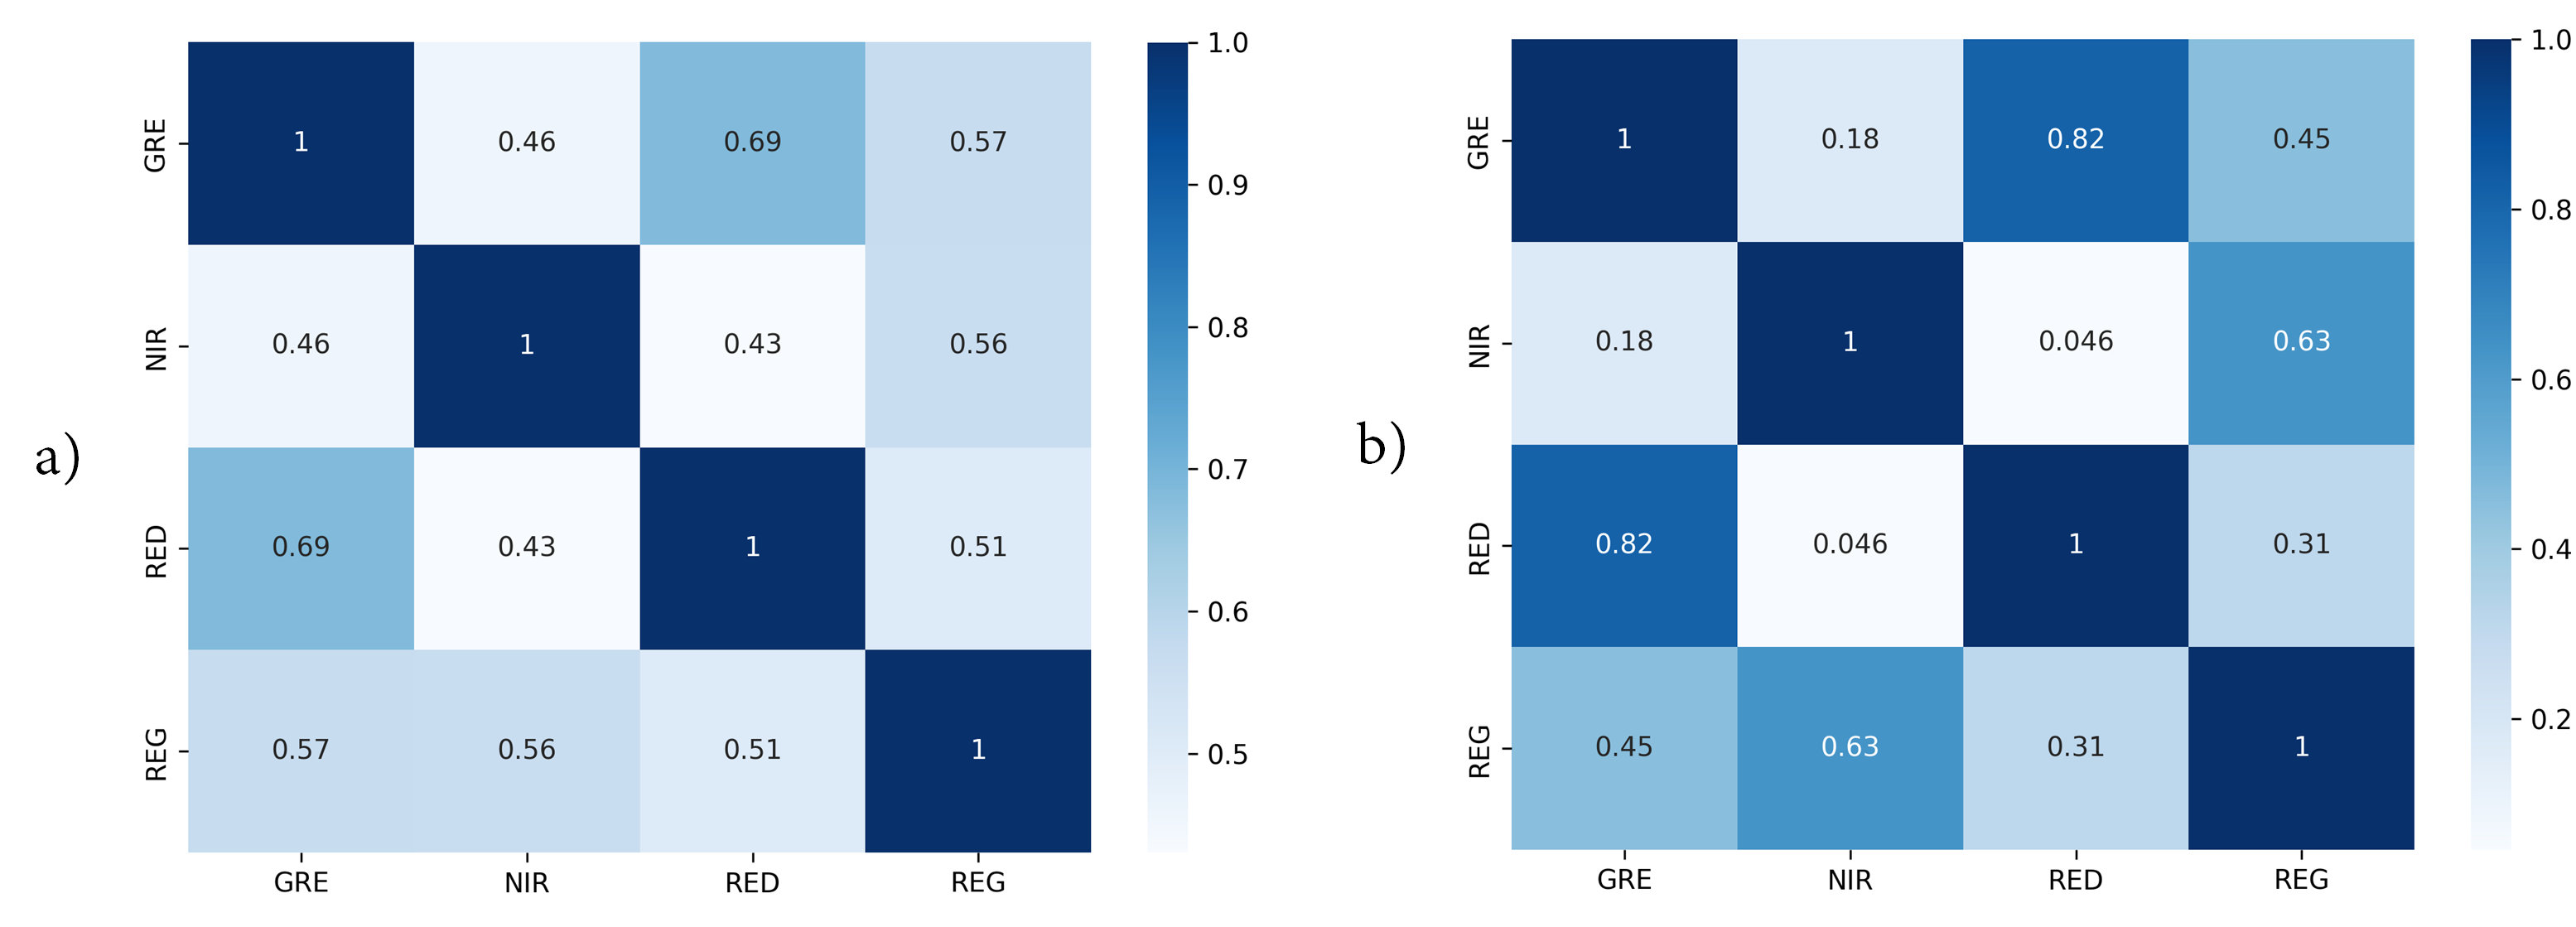
\includegraphics[width=\linewidth]{figs/multi_thermal_projection/results/confusion_matrices.png}
    \caption{Confusion matrix to depict the similarity of multispectral images in the first and second dataset (a) and b), respectively).}
    \label{fig:occlusion_confusion_matrices}
\end{figure*}

Regarding the sought precision, images were aligned using $\epsilon \gets 10^{-5}$ for all the data sources, according to the similarity observed in Figure \ref{fig:ecc_precision}. The similarity was normalized to improve the readability of the chart, though the average intensity differences through the experimental results were observed to be in the order of $1^{-3}$. Lower values (higher exponent) harden the convergence of the \acrshort{ecc} alignment while also increasing the latency in the order of \si{\milli\second}. Hence, an intermediate value that balances both quality and response time was finally used. On the other hand, the number of iterations was established to guarantee that convergence is achieved before reaching such a number. Therefore, a large value such as $\textit{it} \gets 400$ was enough for our case study.

\begin{figure}[ht]
    \centering
    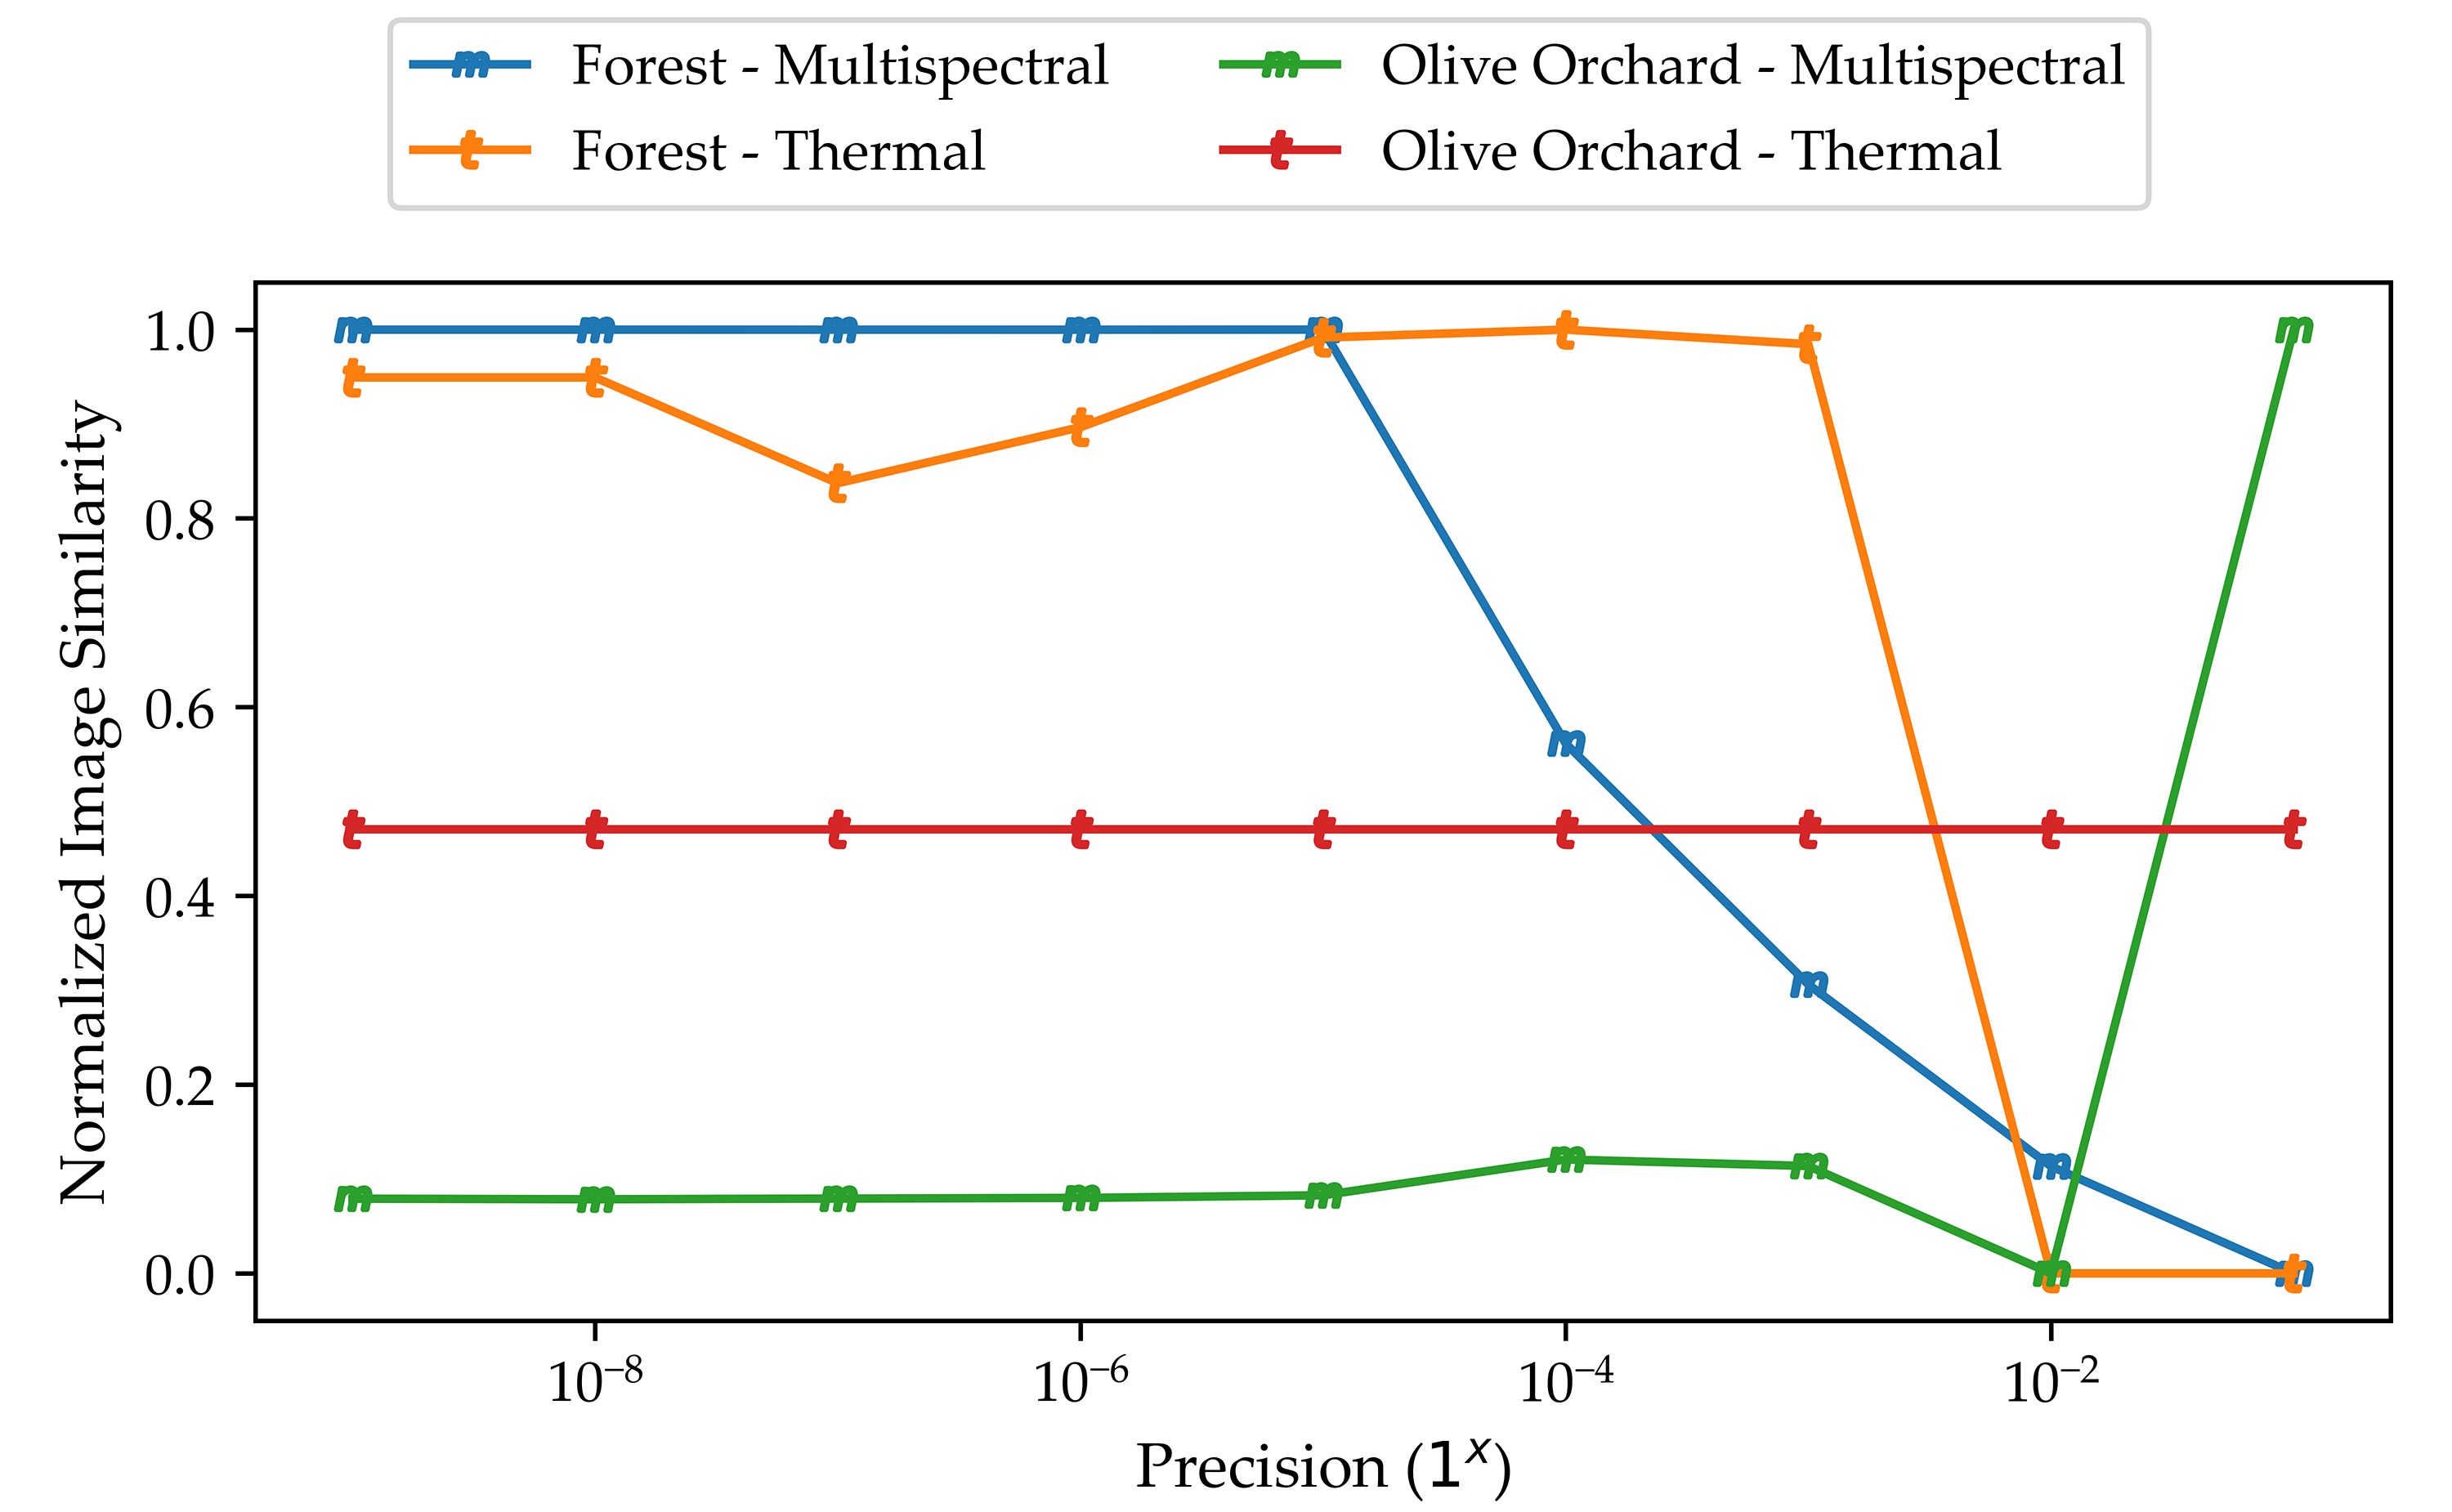
\includegraphics[width=\linewidth]{figs/multi_thermal_projection/results/ecc_precision.png}
    \caption{Image similarity measured after performing the \acrshort{ecc} alignment with a precision equal to $1^x$. Lower values seek the most accurate alignment. The similarity is normalized in [0, 1] for improving the visualization. }
    \label{fig:ecc_precision}
\end{figure}

\subsection{Response time}

First, the response time of commercial solutions was compared against three configurations of our method. The response time is decomposed into three stages: 1) reading the visible point cloud, only for our method, 2) preprocessing stage, including image registration, and 3) reconstruction of the dense point cloud. For commercial software, the second step comprises the finding and matching of image features. The results are shown in Figure \ref{fig:occlusion_results_global_time}, and further insight is provided in Table \ref{table:thermal_results} and \ref{table:multispectral_results}. The response time of our methodology was significantly lower than in the compared commercial solutions, despite the fact that our method reconstructed larger point clouds. This difference is further exploited for \acrshort{gpu}-based solutions and larger datasets since part of the measured latency comes from the allocation of \acrshort{gpu} buffers that are constructed once and reused for several multispectral layers. Thus, the baseline latency from allocation does not increase with a larger number of images. Accordingly, the sorted \acrshort{gpu} solution improves Agisoft Metashape by 77.3\% on average to build thermographic point clouds. The improvement of multispectral reconstruction is 77.26\% with respect to Pix4Dmapper. 

\begin{figure*}[ht]
    \centering
    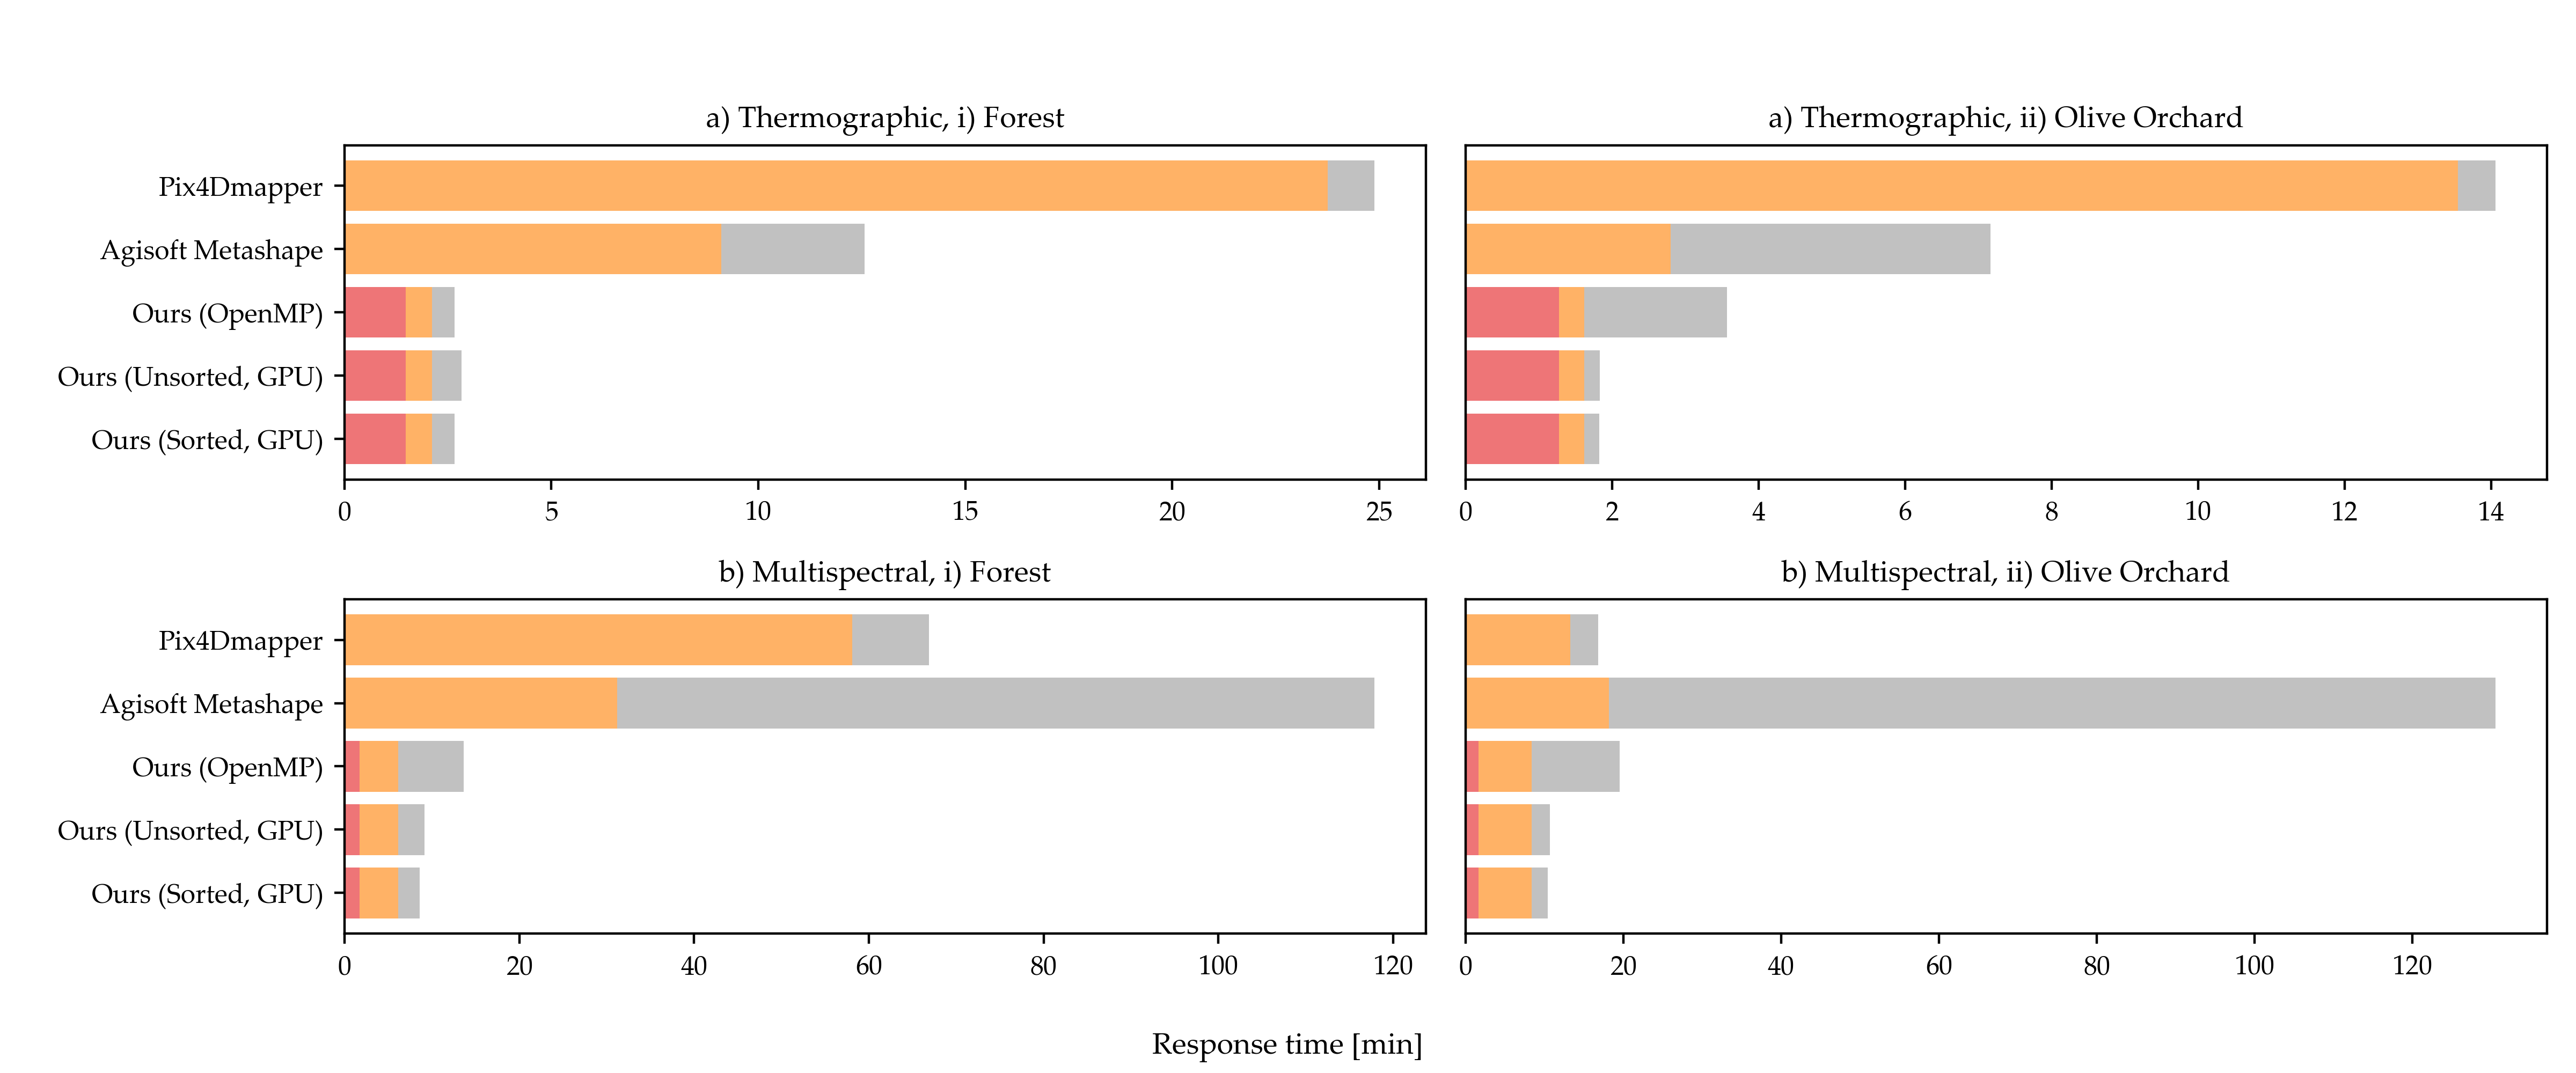
\includegraphics[width=\linewidth]{figs/multi_thermal_projection/results/stacked_global_time.png}
    \caption{Accumulated response time for every data source (1. thermographic and 2. multispectral), study area (a. forestry and b. olive orchard) and solution, including commercial software and configurations of our method. }
    \label{fig:occlusion_results_global_time}
\end{figure*}

\begin{figure*}
    \ContinuedFloat
    \centering
    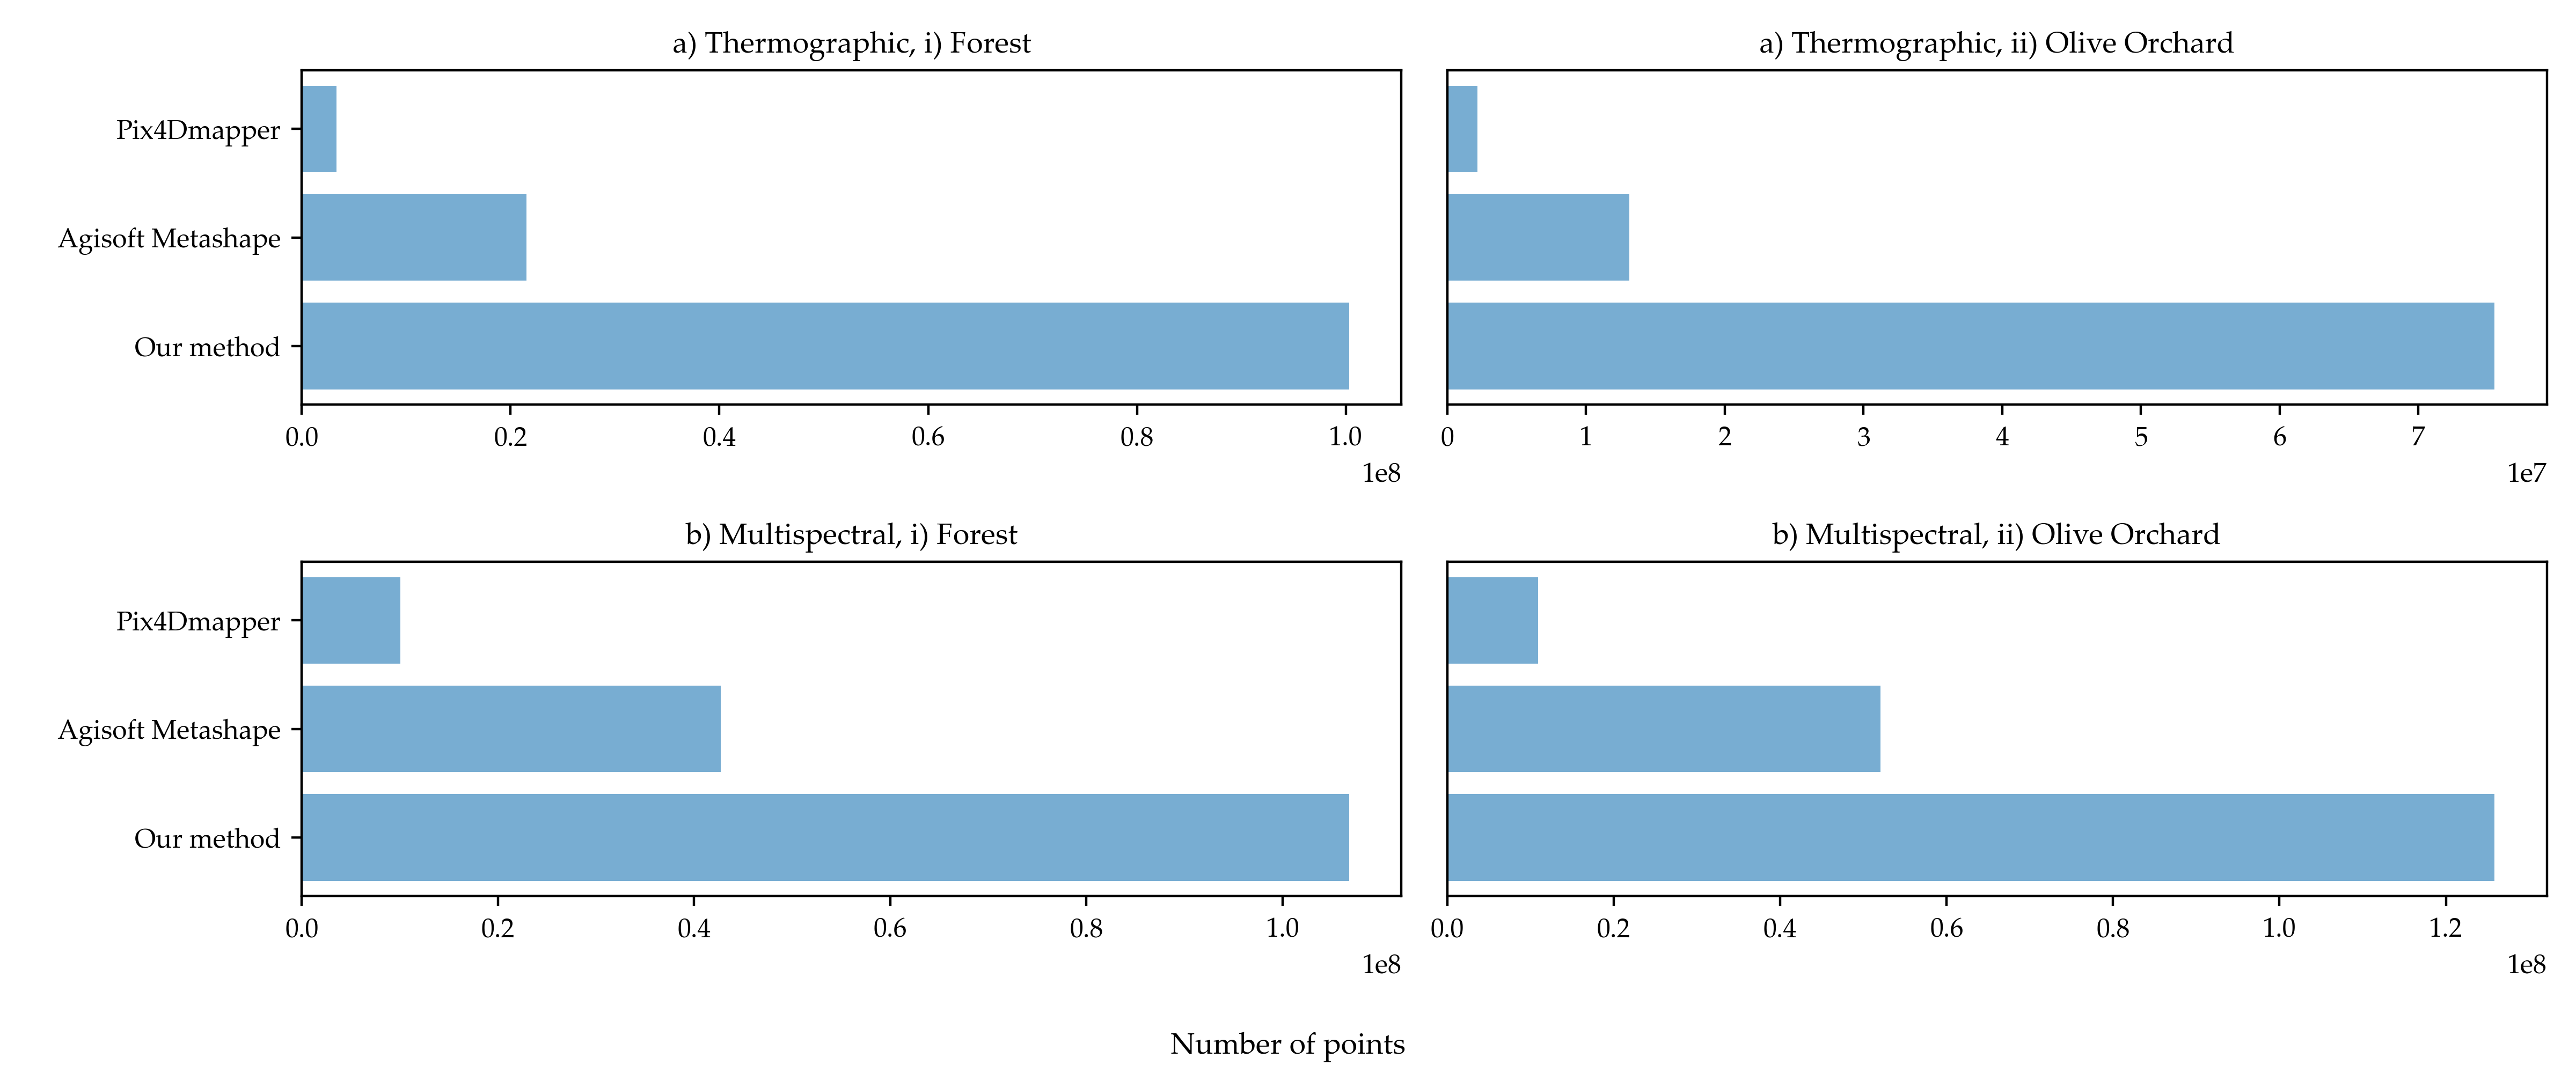
\includegraphics[width=\linewidth]{figs/multi_thermal_projection/results/point_cloud_size.png}
    \caption{Continuation of Figure \ref{fig:occlusion_results_global_time} on the dimensionality of the reconstructed point clouds. }
    \label{fig:occlusion_point_cloud_size}
\end{figure*}

\newcommand\numExperiments{4}

\renewcommand{\arraystretch}{1.3}
\begin{table*}
    \centering
    \footnotesize
    \caption{Numeric results obtained from commercial solutions and different configurations of our approach in two different thermal datasets. The global response time is split into reading point cloud (Stage 1), pre-processing (Stage 2) and densification (Stage 3), i.e., generation of a dense point cloud. }
    \label{table:thermal_results}
    \begin{tabular}{l@{\hskip 0.06in}|lll|l|l|l|l}
    \toprule
    \textbf{Configuration} & \textbf{Stage 1} & \textbf{Stage 2} & \textbf{Stage 3} & \textbf{Latency} & \textbf{Latency/point} & \textbf{\#Points} & \textbf{Matching}\\
    \cmidrule{1-8}
    \multicolumn{8}{c}{Thermal Dataset 1 (Forestry)}\\
    \cmidrule{1-8}
    Pix4Dmapper & - & 23.76 \si{\minute} & 1.13 \si{\minute} & 24.89 \si{\minute} & 449.08 \si{\micro\second}/point & 3,325,454 & 98\%\\
    Agisoft Metashape & - & \textbf{9.10} \si{\minute} & 3.47 \si{\minute} & 12.57 \si{\minute} & 35.05 \si{\micro\second}/point & 21,514,286 & 62.95\%\\
    \cmidrule{1-8}
    OpenMP, No Sort & \multirow{\numExperiments}{*}{1.48 \si{\minute}} & \multirow{\numExperiments}{*}{\textbf{0.64 \si{\minute}}} & 9.77 \si{\minute} & 11.89 \si{\minute} & 6.90 \si{\micro\second}/point & \multirow{\numExperiments}{*}{\textbf{100,322,449}} & \multirow{\numExperiments}{*}{\textbf{99.287\%}}\\
    \acrshort{gpu}, No Sort & & & 0.71 \si{\minute} & 2.83 \si{\minute} & 1.69 \si{\micro\second}/point & &\\
    \acrshort{gpu}, Global Sort & & & \textbf{0.546 \si{\minute}} & \textbf{2.666 \si{\minute}} & \textbf{1.594 \si{\micro\second}/point} & &\\
    %Ours - \acrshort{gpu}, Shuffle Sort & & & \textbf{0.543 \si{\minute}} & \textbf{2.663 \si{\minute}} & \textbf{1.592 \si{\micro\second}/point} & &\\
    \bottomrule
    \toprule
    \multicolumn{8}{c}{Thermal Dataset 2 (Olive orchard)}\\
    \cmidrule{1-8}
    Pix4Dmapper & - & 13.55 \si{\minute} & 0.51 \si{\minute} & 14.06 \si{\minute} & 388.92 \si{\micro\second}/point & 2,169,058 & 90\%\\
    Agisoft Metashape & - & \textbf{2.80} \si{\minute} & 4.37 \si{\minute} & 7.17 \si{\minute} & 32.79 \si{\micro\second}/point & 13,117,583 & \textbf{99.39\%}\\
    \cmidrule{1-8}
    OpenMP, No Sort & \multirow{\numExperiments}{*}{1.28 \si{\minute}} & \multirow{\numExperiments}{*}{\textbf{0.34 \si{\minute}}} & 1.95 \si{\minute} & 3.57 \si{\minute} & 2.83 \si{\micro\second}/point & \multirow{\numExperiments}{*}{\textbf{75,494,967}} & \multirow{\numExperiments}{*}{89.75\%}\\
    \acrshort{gpu}, No Sort & & & 0.217 \si{\minute} & 1.837 \si{\minute} & 1.459 \si{\micro\second}/point & &\\
    \acrshort{gpu}, Global Sort & & & \textbf{0.208 \si{\minute}} & \textbf{1.828 \si{\minute}} & \textbf{1.452 \si{\micro\second}/point} & &\\
    %Ours - \acrshort{gpu}, Shuffle Sort & & & \textbf{0.207 \si{\minute}} & \textbf{1.827 \si{\minute}} & \textbf{1.452 \si{\micro\second}/point} & &\\
    \bottomrule
    \end{tabular}
\end{table*}
\renewcommand{\arraystretch}{1}

\renewcommand{\arraystretch}{1.3}
\begin{table*}
    \centering
    \footnotesize
    \caption{Continuation of Table \ref{table:thermal_results} for multispectral datasets. }
    \label{table:multispectral_results}
    \begin{tabular}{l@{\hskip 0.06in}|lll|l|l|l|l}
    \toprule
    \textbf{Configuration} & \textbf{Stage 1} & \textbf{Stage 2} & \textbf{Stage 3} & \textbf{Latency} & \textbf{Latency/point} & \textbf{\#Points} & \textbf{Matching}\\
    \cmidrule{1-8}
    \multicolumn{8}{c}{Multispectral Dataset 1 (Forestry)}\\
    \cmidrule{1-8}
    Pix4Dmapper & - & 58.11 \si{\minute} & \textbf{8.76} \si{\minute} & 66.87 \si{\minute} & 398.35 \si{\second}/point & 10,071,939 & 97\%\\
    Agisoft Metashape & - & \textbf{31.22} \si{\minute} & 86.64 \si{\minute} & 117.86 \si{\minute} & 165.49 \si{\micro\second}/point & 42,731,004 & 67.74\%\\
    \cmidrule{1-8}
    OpenMP, No Sort & \multirow{\numExperiments}{*}{1.71 \si{\minute}} & \multirow{\numExperiments}{*}{\textbf{4.45 \si{\minute}}} & 7.50 \si{\minute} & 13.66 \si{\minute} & 7.67 \si{\micro\second}/point & \multirow{\numExperiments}{*}{\textbf{106,780,612}} & \multirow{\numExperiments}{*}{\textbf{100\%}}\\
    \acrshort{gpu}, No Sort & & & 2.99 \si{\minute} & 9.15 \si{\minute} & 5.14 \si{\micro\second}/point & &\\
    \acrshort{gpu}, Global Sort & & & \textbf{2.42 \si{\minute}} & \textbf{8.58 \si{\minute}} & \textbf{4.82 \si{\micro\second}/point} & &\\
    %Ours - \acrshort{gpu}, Shuffle Sort & & & \textbf{2.40 \si{\minute}} & \textbf{8.56 \si{\minute}} & \textbf{4.80 \si{\micro\second}/point} & &\\
    \bottomrule
    \toprule
    \multicolumn{8}{c}{Multispectral Dataset 2 (Olive orchard)}\\
    \cmidrule{1-8}
    Pix4Dmapper & - & \textbf{13.3} \si{\minute} & \textbf{3.5} \si{\minute} & 16.8 \si{\minute} & 92.56 \si{\micro\second}/point & 10,889,523 & \textbf{100\%}\\
    Agisoft Metashape & - & 18.15 \si{\minute} & 112.36 \si{\minute} & 130.51 \si{\minute} & 150,52 \si{\micro\second}/point & 52,021,396 & \textbf{100\%}\\
    \cmidrule{1-8}
    OpenMP, No Sort & \multirow{\numExperiments}{*}{1.67 \si{\minute}} & \multirow{\numExperiments}{*}{\textbf{6.69} \si{\minute}} & 11.19 \si{\minute} & 19.55 \si{\minute} & 9.32 \si{\micro\second}/point & \multirow{\numExperiments}{*}{\textbf{125,857,793}} & \multirow{\numExperiments}{*}{99.934 \%}\\
    \acrshort{gpu}, No Sort & & & 2.31 \si{\minute} & 10.67 \si{\minute} & 5.08 \si{\micro\second}/point & &\\
    \acrshort{gpu}, Global Sort & & & \textbf{2.08 \si{\minute}} & \textbf{10.44 \si{\minute}} & \textbf{4.97 \si{\micro\second}/point} & &\\
    %Ours - \acrshort{gpu}, Shuffle Sort & & & 2.09 \si{\minute} & 10.45 \si{\minute} & 4.98 \si{\micro\second}/point & &\\
    \bottomrule
    \end{tabular}
\end{table*}
\renewcommand{\arraystretch}{1}

The tests were performed with a $z$-buffer with $d \gets 10$, which was shown to balance latency and point cloud dimensionality. Larger values of $d$ involve higher data transfers, while also risking to include background points with foreground data. Otherwise, lower values of $d$ reduce the dimensionality of point clouds at the expense of minimizing the latency from data transfers. Based on this, $d \gets 1$ would provide the baseline improvement of the \acrshort{ecc} method with respect to the recognition of feature points in images to build a sparse point cloud. Both procedures iterate over the whole dataset, whereas the former only evaluates a set of paired images instead of surrounding images. This improvement is considerably lowered for multispectral images since \acrshort{ecc} is performed up to five times. 

\subsubsection{Comparison of \acrshort{opengl} and \acrshort{cuda} solutions}

Table \ref{table:cuda_opengl_occlusion_response_time} shows the response time measured from data transfers and the occlusion-aware projection. The single batch configuration loads the whole point cloud in a single buffer if the maximum size of an \acrshort{ssbo} is below the maximum allocatable \acrshort{gpu} memory. Otherwise, it works as the \textbf{Multiple batches} approach does. On the other hand, the \acrshort{cuda} framework was able to handle the largest point cloud (271M points) in a single buffer. The reported results are the lowest timed response time from five different tests. The measured latency in Table \ref{table:cuda_opengl_occlusion_response_time} and Figure \ref{fig:cuda_opengl_occlusion_response_time} show that compute shaders significantly improve the response time obtained using the traditional rendering pipeline and \acrshort{cuda}. Also, the rendering pipeline offered slightly better results than \acrshort{cuda} for the single-batch workflow. Regarding the use of multiple batches, both \acrshort{opengl}-based approaches worsened their performance in comparison with previous tests. In contrast, the \acrshort{cuda} version obtained similar results to the previously measured latency. 

\begin{figure}[ht]
    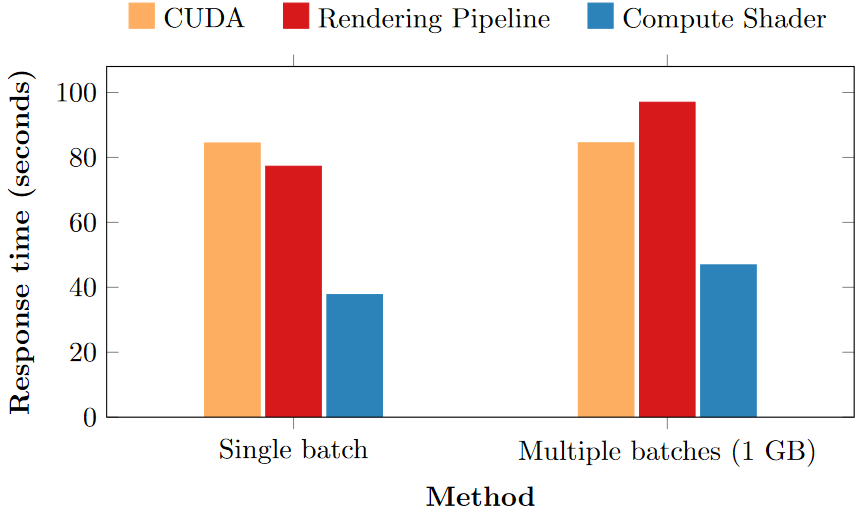
\includegraphics[width=.8\linewidth]{figs/multi_thermal_projection/results/response_time_cuda_opengl.png}
    \caption{Latency in seconds for \acrshort{opengl} and \acrshort{cuda} approaches, using a point cloud with 271M points and 1352 viewpoints).}
    \label{fig:cuda_opengl_occlusion_response_time}
\end{figure}

\renewcommand{\arraystretch}{1.2}
\begin{table*}[htb]
\centering
\caption{Response time of methodologies using \acrshort{opengl} and \acrshort{cuda}, including data transfers between \acrshort{cpu} and \acrshort{gpu}.}
\label{table:cuda_opengl_occlusion_response_time}
\begin{tabular}{llllll}
    \toprule
    \multicolumn{2}{c}{} & \multicolumn{4}{c}{\textbf{Environment}} \\
    \cmidrule{3-6}
    \multicolumn{2}{c}{} & \multicolumn{2}{c}{\textbf{180 cameras}} & \multicolumn{2}{c}{\textbf{1352 cameras}}\\
    \cmidrule{3-6}
    \multicolumn{2}{c}{\textbf{Proposed methods}} & 66M points & 271M points & 66M points & 271M points\\
    \midrule
    \multirow{3}{*}{Single batch} & \acrshort{cuda} & 2.97s & 10.30s & 23.58s & 84.45s\\
    & Rendering pipeline & 2.52s & 10.38s & 20.70s & 77.28s\\
    & Compute shaders & \textbf{1.43s} & \textbf{6.21s} & \textbf{8.90s} & \textbf{37.75s}\\
    \hline
    \multirow{3}{*}{Multiple batches (1 GB)} & \acrshort{cuda} & 3.22s & 11.19s & 25.42s & 84.50s\\
    & Rendering pipeline & 3.71s & 13.35s & 29.15s & 96.99s\\
    & Compute shaders & \textbf{2.57s} & \textbf{7.61s} & \textbf{18.16s} & \textbf{46.90s}\\
    \bottomrule
\end{tabular}
\end{table*}
\renewcommand{\arraystretch}{1}

%As depicted in Figure \arraybackslash, the best configuration of our method outperforms other commercial solutions in terms of both response time and point cloud size. Agisoft Metashape also presents a competitive performance, although the point cloud with maximum quality solely consists of 18M points. On the other hand, the baseline of our method is an \acrshort{rgb} point cloud with 98M points. With $d = 10$, we achieve a thermal point cloud with 84M points, whereas the response time is similar to the \acrshort{cuda}-based approach of Agisoft Metashape.

\subsection{Point cloud size and normalized response time}

The proposed method is included as part of a pipeline where dense point clouds of \acrshort{rgb} and alternative data sources are jointly reconstructed. In this scenario, the first point cloud is considerably larger than those obtained with imagery of lower resolution and less recognizable features. From this baseline, the number of points of the \acrshort{rgb} point cloud is reduced according to their visibility from the whole set of camera viewpoints and the depth buffer's resolution. Still, most of them are preserved and linked to data interpolated from thermal and multispectral imagery in our case study. 

Point clouds reconstructed from multispectral images are dense due to the provided variety of reflectance and the higher number of recognized features. However, the higher sparsity of thermal point clouds is observed in Figure \ref{fig:occlusion_point_cloud_size}. For the thermographic datasets, our method increases the point cloud size by 366.3\% (forest) and 475.52\% (olive orchard) with respect to Agisoft Metashape. In this regard, this commercial solution reconstructs the densest point clouds from the compared software, both for multispectral and thermal imagery. Despite this, it is significantly slower for larger datasets such as the multispectral. For the latter data source, the size increases by 149.89\% (forest) and 141.93\% (olive orchard) also in comparison with Agisoft Metashape.

Previous results based on global latency present a wider gap if they are normalized according to the point cloud's dimensionality. The normalized latency of our best method improves the results of the best commercial solution by 95.51\% and 96.9\% on average for thermal and multispectral images, respectively. 

\subsection{Overall comparison}

The results of the four datasets and the five compared methods are summarized in Figure \ref{fig:occlusion_normalized_features}. The global latency and point cloud size features are normalized in $[0, 1]$. The first feature must be minimized, whereas the second one ought to be maximized to provide a better reconstruction of the target scenario. According to this figure, the three proposed methods present an outstanding performance in terms of response time and point cloud dimensionality. These are followed by Agisoft Metashape, which is considerably slower, albeit generating larger results than the last alternative, Pix4Dmapper.

\begin{figure}[ht]
    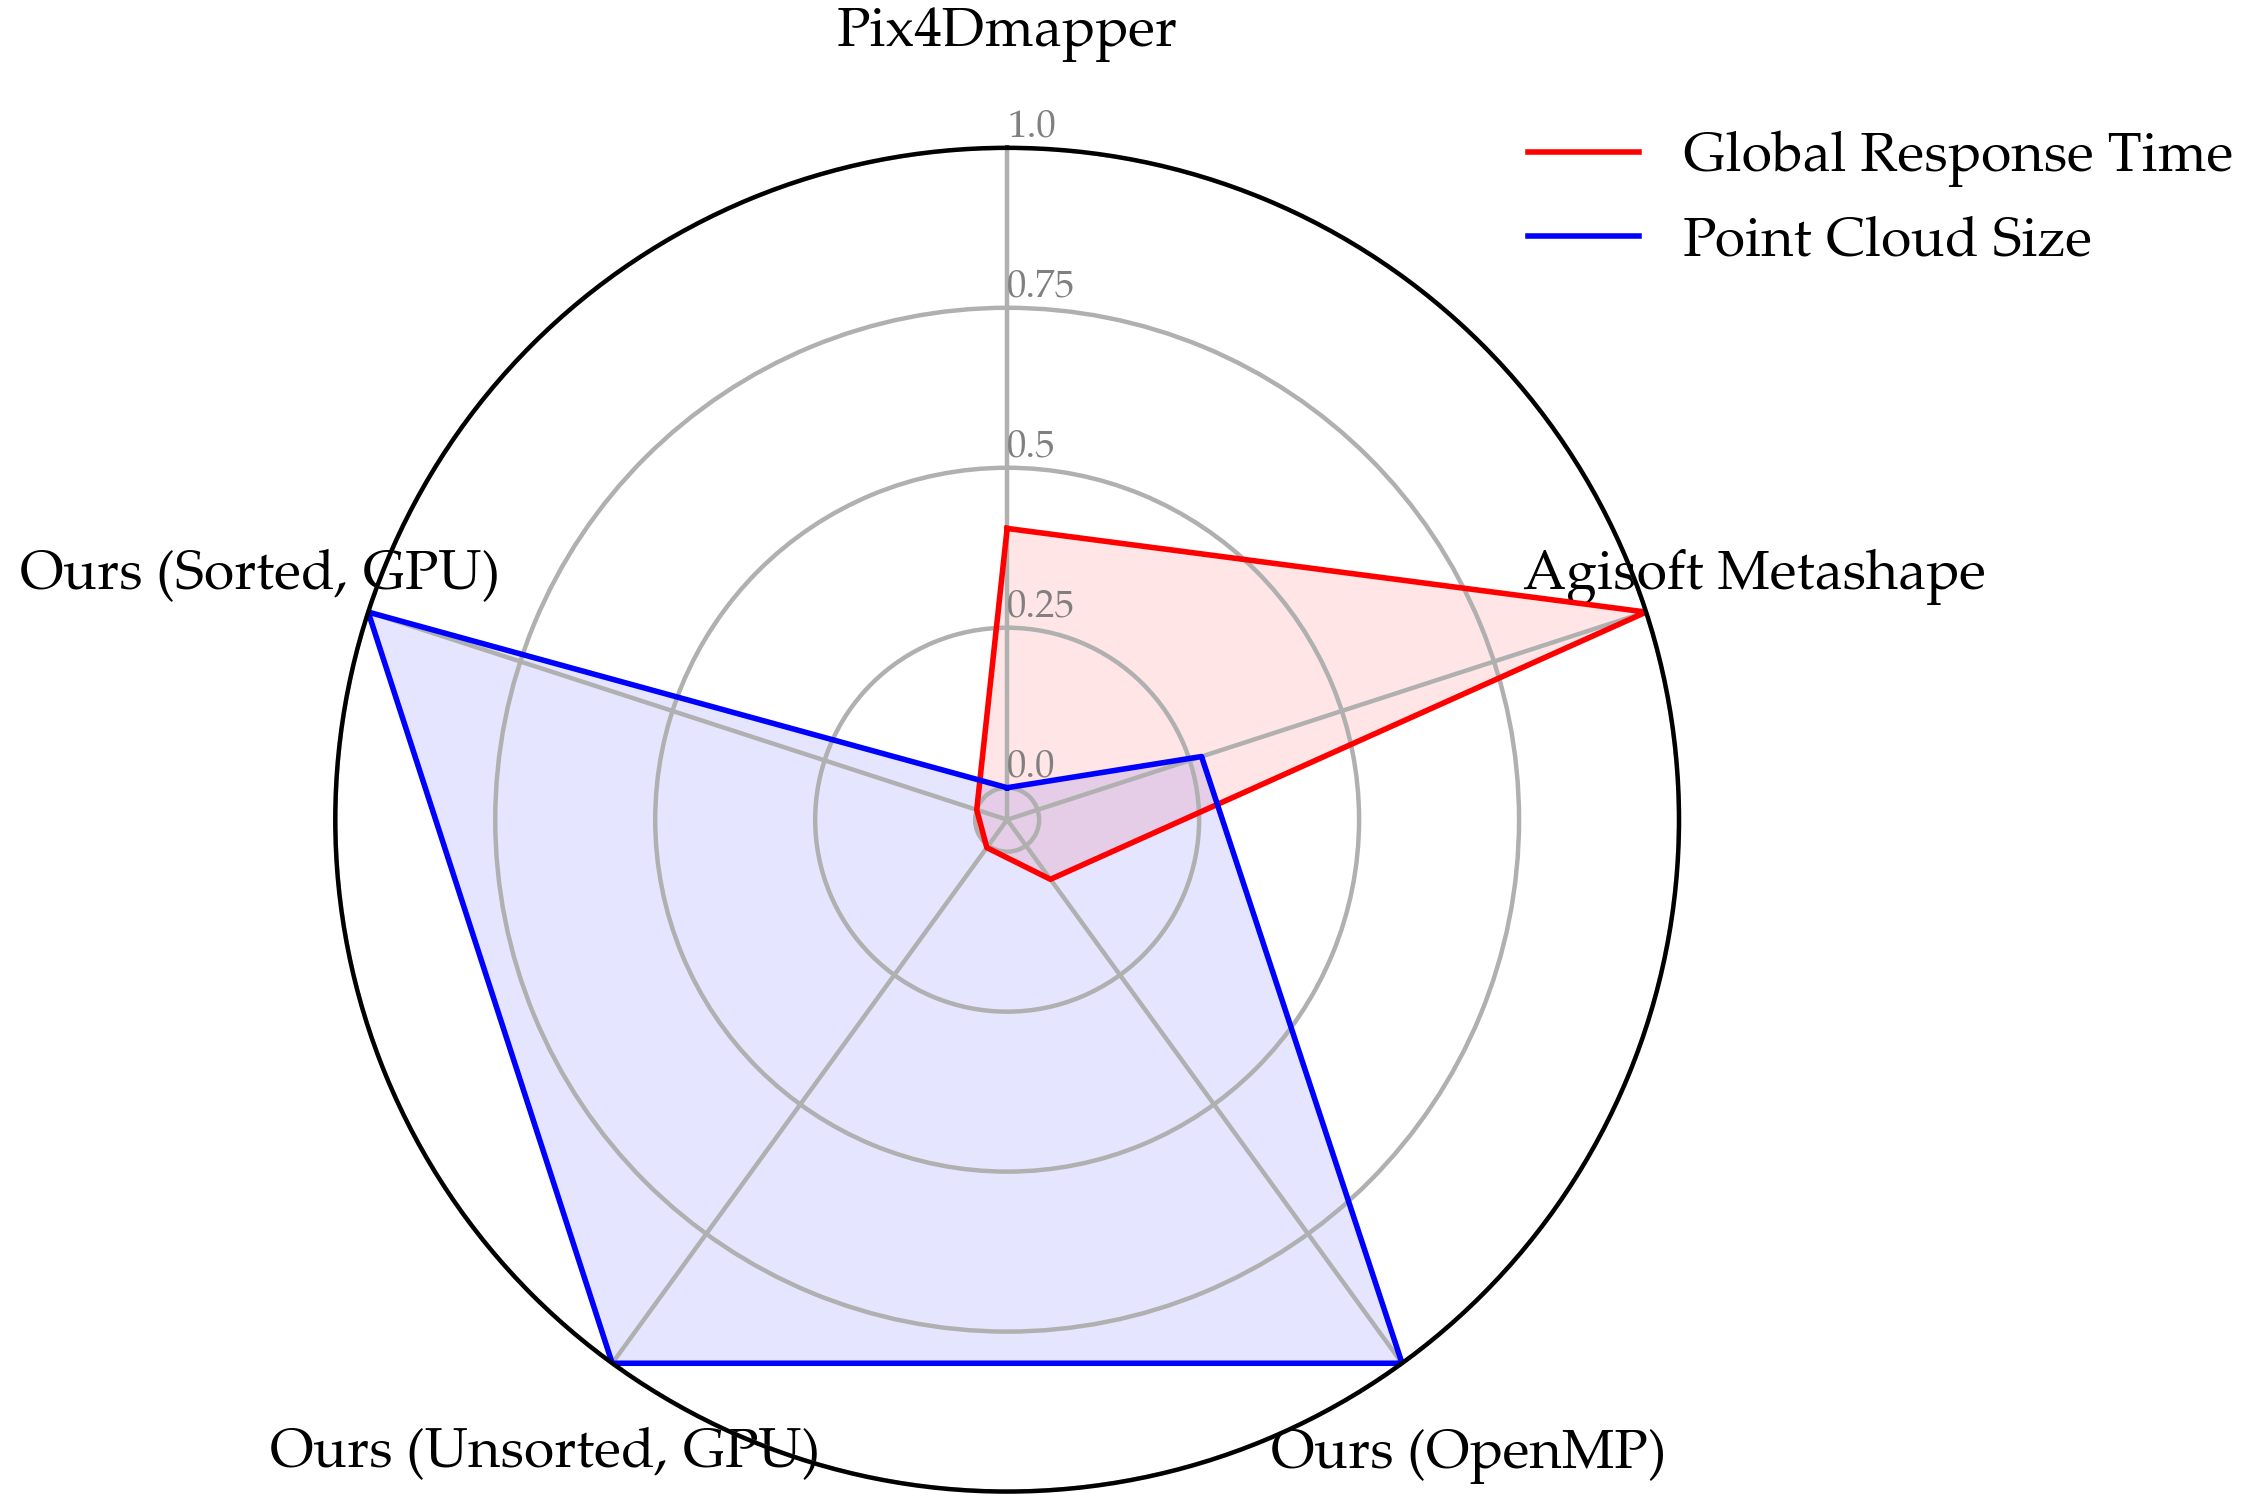
\includegraphics[width=.8\linewidth]{figs/multi_thermal_projection/results/normalized_features.png}
    \caption{Average response time and point cloud size obtained by commercial software and three versions of the proposed method.}
    \label{fig:occlusion_normalized_features}
\end{figure}

\subsection{Data shuffling in \acrshort{gpu}}

\begin{figure*}
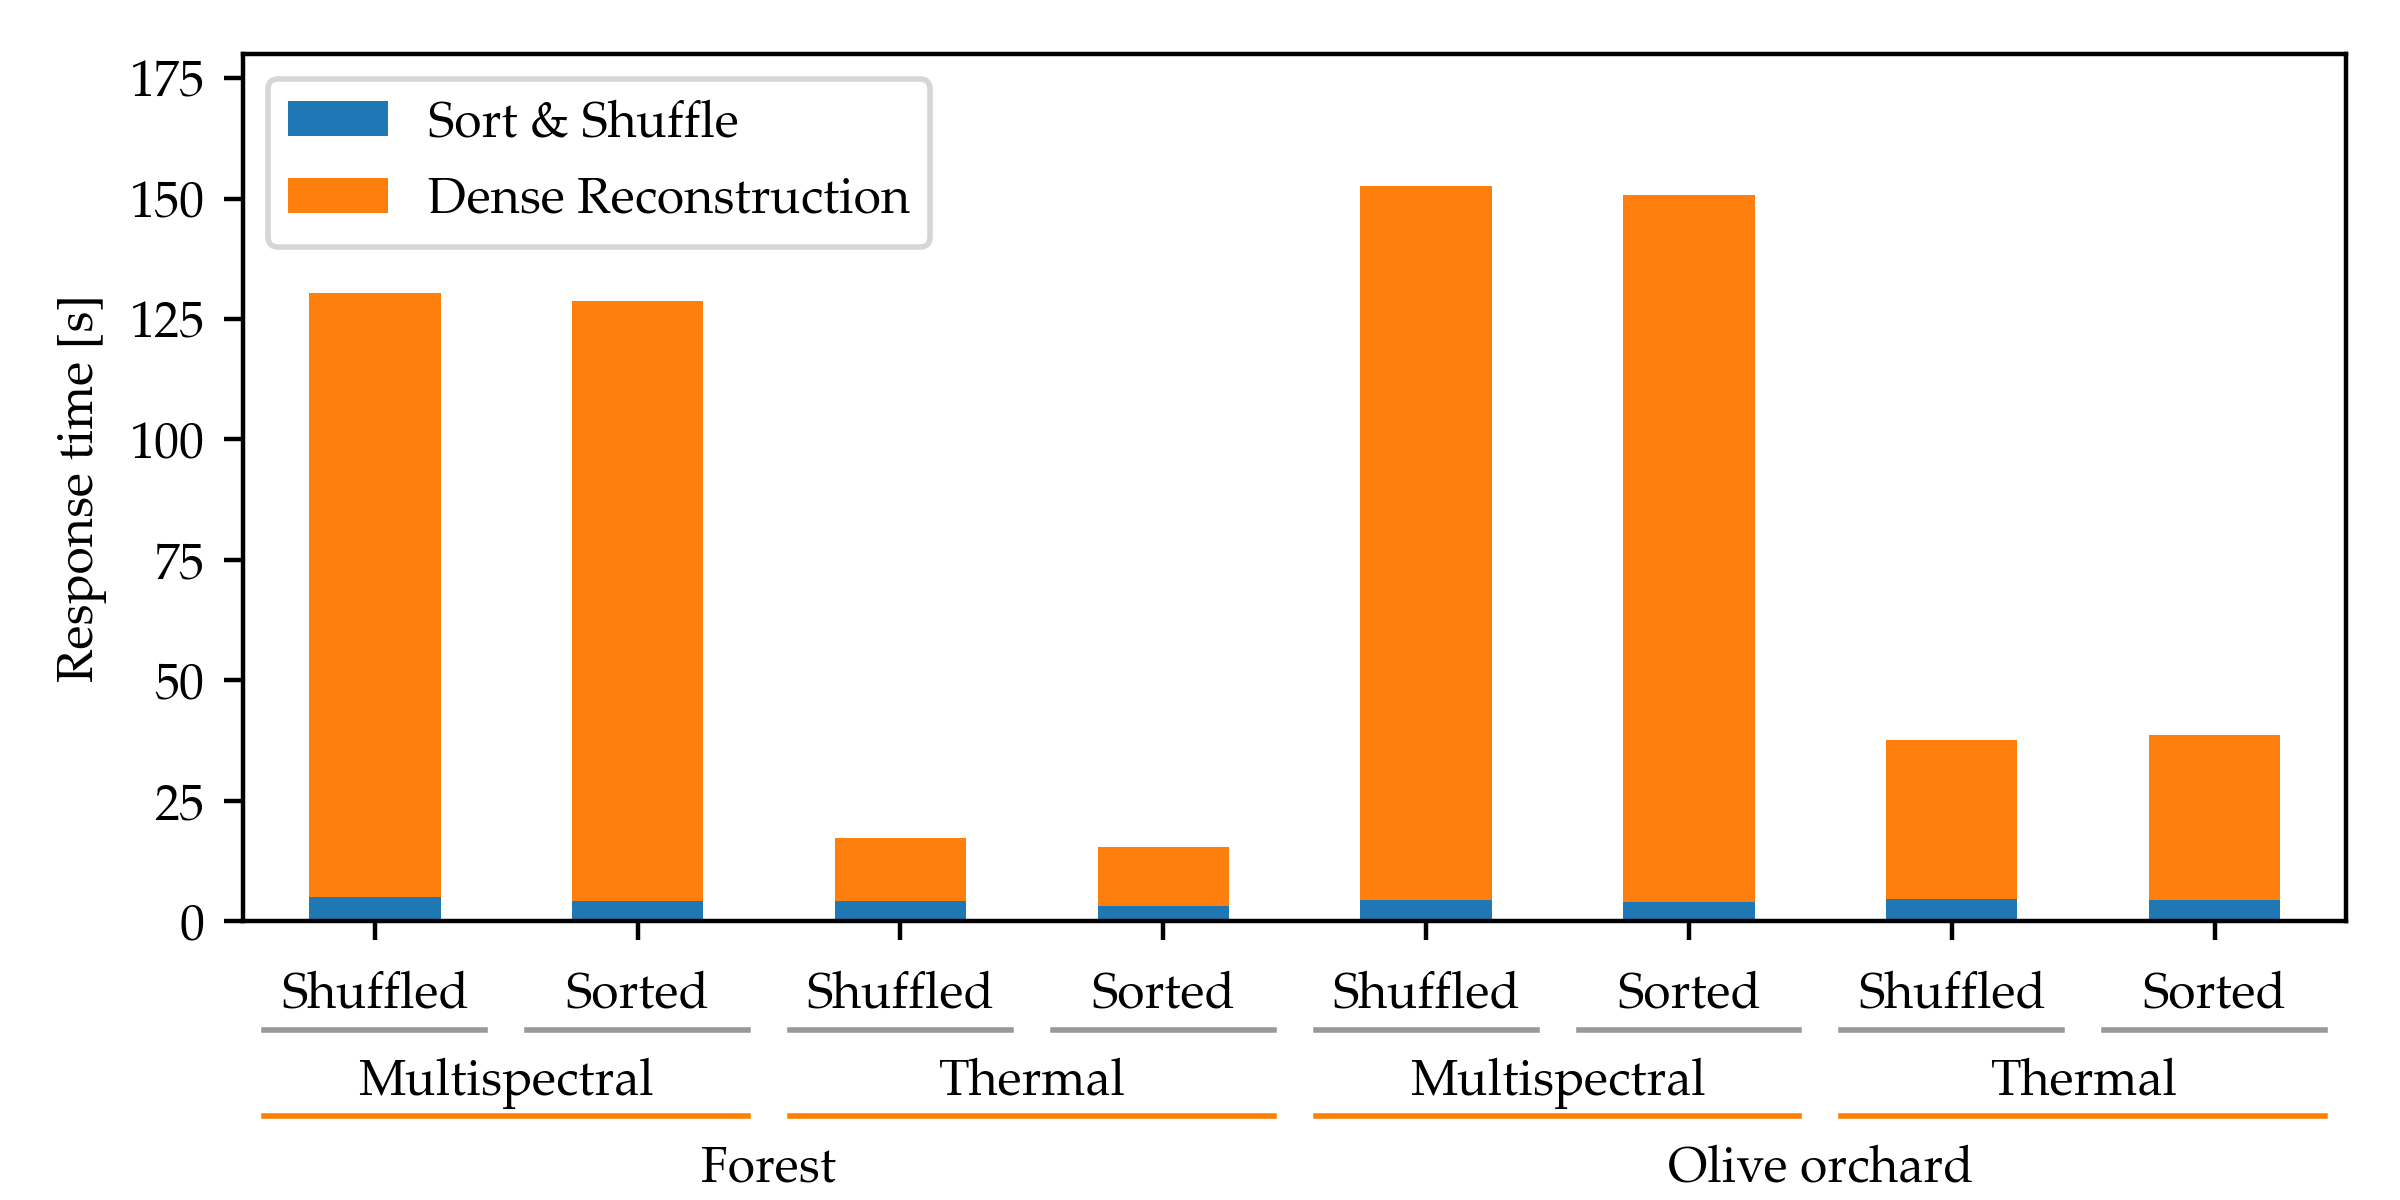
\includegraphics[width=.75\linewidth]{figs/multi_thermal_projection/results/stacked_stage_response_time.png}
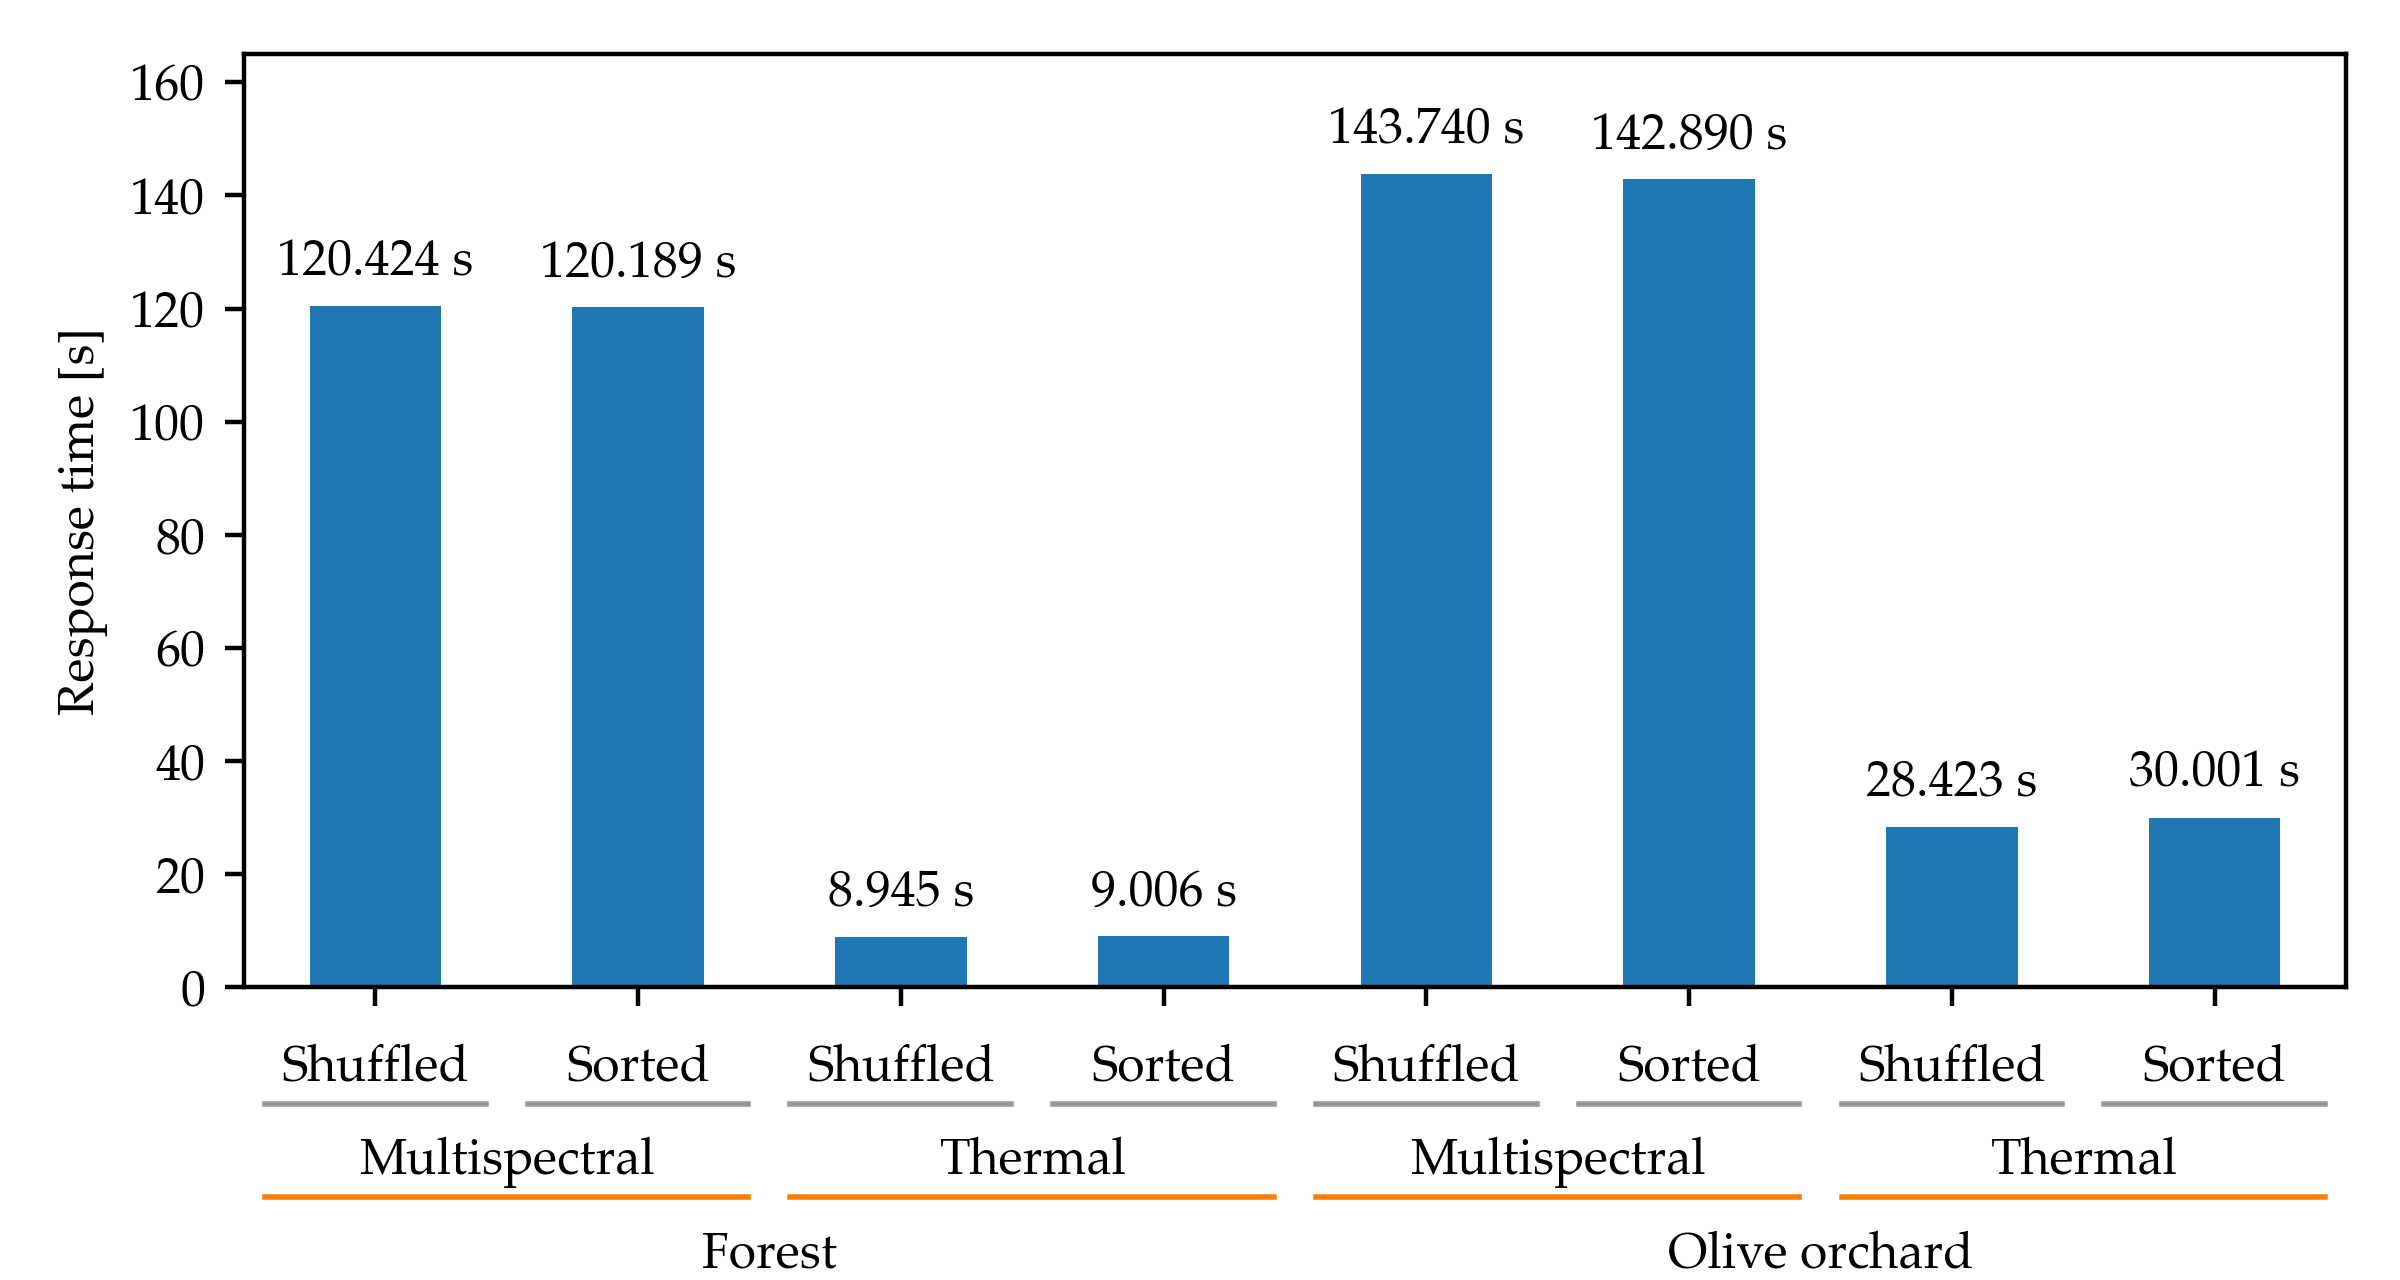
\includegraphics[width=.75\linewidth]{figs/multi_thermal_projection/results/shuffled_response_time.png}
\caption{Comparison of performance of the dense reconstruction stage using sorted \& shuffled data and globally sorted data. The first image compares the overall latency of the dense reconstruction, whereas the second image only compares the projection procedure.}
\label{fig:shuffle_comparison}
\end{figure*}

As stated by previous work \cite{schutz_rendering_2021, kerbl_effective_2017}, specific \acrshort{gpu} patterns are used by manufacturers to distribute the workload among thread groups. This knowledge can help to further reduce the latency of \acrshort{gpu}-based solutions, in comparison with globally sorted point clouds. Thus, the objective is to shuffle points in batches to balance the workload of every workgroup. As the outcome of a batch is expected to depend on the camera viewpoint, the data shuffling ought to help to reduce latency by distributing visible and non-visible points. To this end, a comparison of data shuffled or not after being sorted was conducted, with groups of size $g \gets 32$. The results are depicted in Figure \ref{fig:shuffle_comparison} by splitting the latency into the Sort \& Shuffle and Reconstruction stages. Numeric results are also annotated in Table \ref{table:shuffling_results}.

\renewcommand{\arraystretch}{1.2}
\begin{table*}
    \sffamily\footnotesize
    \centering
    \caption{Latency of the first two stages if 1) it is the first load or 2) binary data has already been stored as a result of a previous load. }
    \label{table:shuffling_results}    
    \begin{tabular}{l@{\hskip 0.07in}|ll|ll}
    \toprule
     & \multicolumn{2}{c}{Global sort} & \multicolumn{2}{c}{Shuffled sort ($g \gets 32$)}\\
    \cmidrule{1-5}
    \textbf{Dataset} & Point cloud sort & Dense reconstruction &  Point cloud sort & Dense reconstruction\\
    \cmidrule{1-5}
    a) Thermal, i) Forest & \textbf{0.071 \si{\minute}} & 0.500 \si{\minute}
    & 0.076 \si{\minute} & \textbf{0.473} \si{\minute}\\
    \cmidrule{1-5}
    a) Thermal, ii) Olive orchard & \textbf{0.052 \si{\minute}} & 0,150 \si{\minute}
    & 0.052 \si{\minute} & \textbf{0.149 \si{\minute}}\\
    \cmidrule{1-5}
    b) Multispectral, i) Forest & \textbf{0.065 \si{\minute}} & \textbf{2.381 \si{\minute}}
    & 0.074 \si{\minute} & 2.395 \si{\minute}\\
    \cmidrule{1-5}
    b) Multispectral, ii) Olive orchard & \textbf{0.071 \si{\minute}} & \textbf{2.003 \si{\minute}}
    & 0.082 \si{\minute} & 2.007 \si{\minute}\\
    \bottomrule
    \end{tabular}
\end{table*}
\renewcommand{\arraystretch}{1}

To provide a better insight into the data shuffling, the second image shows only the response time from the dense reconstruction. The shuffled ordering also involves global sorting prior to organizing the point cloud into batches. Thus, the Sort \& Shuffle procedure is more time-consuming than solely sorting. Accordingly, the summed response time of the Shuffled version is higher for every configuration whether both stages are included. Otherwise, the results offer slight changes if only the reconstruction stage is considered. It is observed that data shuffling effectively helps to reduce latency in smaller point clouds (thermographic), whereas larger point clouds worsen the latency obtained by the global sort. Unlike previous studies, the proposed case study is very unbalanced for individual viewpoints. From hundreds of millions of points, only a few million are visible from a camera viewpoint. Thus, the workload balancing was not effective. Even if so, the Shuffle stage increases the latency for a one-time process, thus making it not worth it. Instead, repetitive tasks such as rendering are more likely to benefit from the use of this technique.

\subsection{Visual results}

Table \ref{table:visual_results} shows the rendering of multispectral and thermographic point clouds obtained by the three compared solutions. In this regard, both commercial solutions are observed to reconstruct incomplete and erroneous geometry for thermographic data. Instead, our method projects these data over an \acrshort{rgb} point cloud that is accurately reconstructed. Multispectral imagery presents higher dimensionality and more recognized features, thus leading to better reconstructions even for commercial software, regardless of the small point density. Hence, the reconstructed multispectral point clouds are similar among all the compared methods. The main drawback of multispectral point clouds reconstructed with photogrammetry is the existence of gaps, which are much less frequent in \acrshort{rgb} point clouds despite vegetation being hardly reconstructed. 

\subsection{Binary data}

Previous results are measured by 1) loading a Polygon File Format (\acrshort{ply}) point cloud, 2) reading \acrshort{tiff} and \acrshort{jpeg} images and 3) reconstructing the dense point cloud from previous data. However, these are known to be time-consuming stages that can be treated differently after the first load. First, point clouds are stored in binary file format. Similarly, the image alignment results can be stored in binary files. Once aligned, \acrshort{rgb} imagery is not loaded again. Finally, the reconstructed point cloud is stored as an additional colour to be attached to previously stored binary point clouds. Figure \ref{fig:occlusion_binary_response_time} compares the latency of binary and non-binary reading of the first two stages. The latency from the dense reconstruction is equal to the response time of the first stage since they load point clouds of the same size. The numeric data is shown in Table \ref{table:binary_results}. Thus, the proposed procedure is shown to be very time-consuming, yet more efficient than current solutions, though it can be sped up after computing the results for the first time.

\begin{figure}[ht]
    \centering
    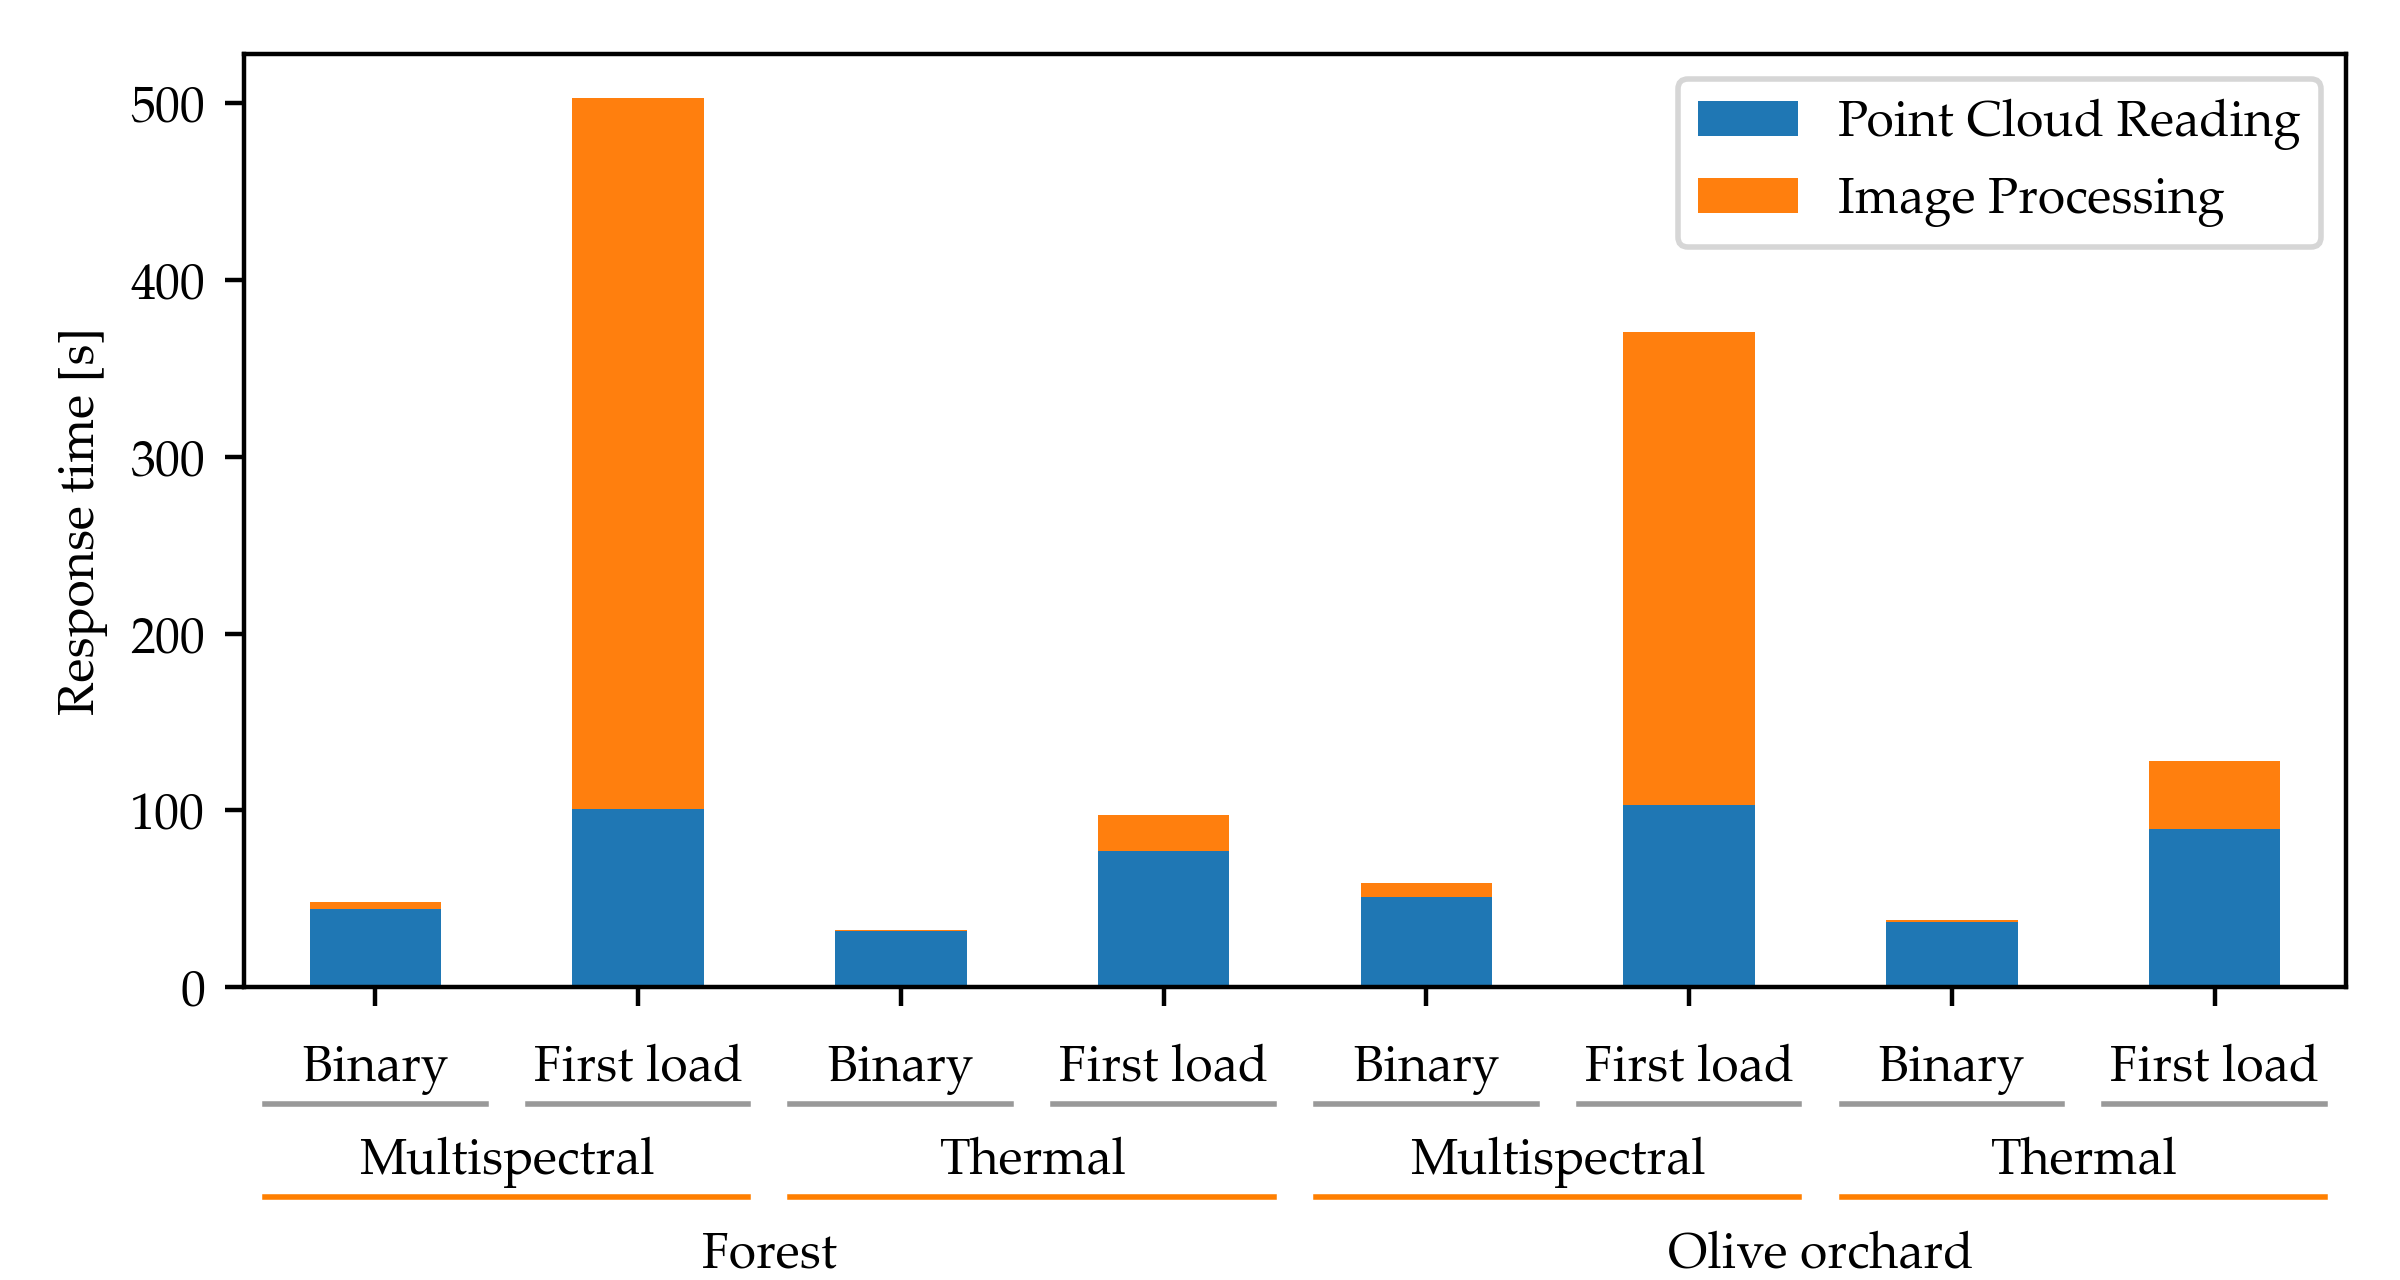
\includegraphics[width=\linewidth]{figs/multi_thermal_projection/results/binary_response_time.png}
    \caption{Comparison of latency measured from the first two stages of our method in the first and subsequent launches (loading calculated data from binary files).}
	\label{fig:occlusion_binary_response_time}
\end{figure}

\renewcommand{\arraystretch}{1.2}
\begin{table*}
    \sffamily
    \centering
    \caption{Response time of the first two stages if 1) it is the first load or 2) binary data has already been stored as a result of a previous load. Stage 1 refers to point cloud reading, whereas Stage 2 involves the image processing prior to the dense reconstruction. }
    \label{table:binary_results}
    \begin{tabular}{l|llll}
    \toprule
    & \multicolumn{2}{c}{Binary} & \multicolumn{2}{c}{First load}\\
    \cmidrule{1-5}
    \textbf{Dataset} & \textbf{Stage 1} & \textbf{Stage 2} & \textbf{Stage 1} & \textbf{Stage 2}\\
    \cmidrule{1-5}
    a) Thermal, i) Forest & \textbf{0.61 \si{\minute}} & \textbf{0.01 \si{\minute}} & 1.48 \si{\minute} & 0.64 \si{\minute}\\
    \cmidrule{1-5}
    a) Thermal, ii) Olive orchard & \textbf{0.52 \si{\minute}} & \textbf{0.01 \si{\minute}} & 1.28 \si{\minute} & 0.34 \si{\minute}\\
    \cmidrule{1-5}
    b) Multispectral, i) Forest & \textbf{0.85 \si{\minute}} & \textbf{0.12 \si{\minute}} & 1.71 \si{\minute} & 4.45 \si{\minute}\\
    \cmidrule{1-5}
    b) Multispectral, ii) Olive orchard & \textbf{0.73 \si{\minute}} & \textbf{0.06 \si{\minute}} & 1.67 \si{\minute} & 6.69 \si{\minute}\\
    \bottomrule
    \end{tabular}
\end{table*}
\renewcommand{\arraystretch}{1}

\section{Conclusions and future work}

Reconstructing multiple 3D point clouds is a common task in surveying work, and it often involves not only visible imagery but also other sensors that provide additional information about the studied field. Therefore, reconstructing 3D point clouds from multiple data sources, such as thermal and multispectral, can be accomplished by leveraging the previous \acrshort{rgb} reconstructions. While commercial software can perform these tasks, several drawbacks were identified, including high response time, low point density, and incorrect estimations without additional knowledge, such as ground control points (\acrshort{gcp}s). The latter issue arises because thermal and multispectral imagery have lower dimensionality and more defects than visible imagery, making it more challenging to recognize image features.

An accelerated projection-based methodology was proposed for integrating reconstructed thermal and multispectral 3D point clouds. The process began with the reconstruction of \acrshort{rgb} point clouds using traditional software. Then, the subsequent reconstructions were performed with significantly lower latency (approximately -77\%), resulting in point clouds that were more than 140\% larger than the initial ones. When normalized according to point cloud size, our method improved latency results by over 95\%. Despite both commercial software and our method using \acrshort{gpu}-accelerated procedures, ours outperformed two widely-used solutions in terms of response time and size.

Although our proposed approach demonstrated improved performance in terms of latency and point cloud size, the parallelism was mainly addressed with \acrshort{glsl}, which provides limited flexibility and control of the execution pipeline, such as overlapping data transfers and thread logic. Additionally, it runs on a single \acrshort{gpu}, thus restricting scalability. Therefore, a future direction is to evaluate our \acrshort{gpgpu} solution over the \acrshort{cuda} framework, which offers more control over the execution pipeline and the possibility to use multiple \acrshort{gpu}s for higher scalability. In addition, our multi-layer point cloud could be further extended by integrating other data sources, such as hyperspectral datasets. Finally, instead of performing the projection over \acrshort{rgb} point clouds, \acrshort{lidar} point clouds could be used to replace the first with a more geometrically accurate product.

\begin{table*}[htb]
    \centering
    \caption{Graphic results of the dense reconstruction computed by 1) Agisoft Metashape, 2) Pix4Dmapper and 3) our method. Multispectral point clouds are rendered with the Green layer. }
    \label{table:visual_results}  
    \newcommand\imageTableSize{0.44\textwidth}
    \begin{tabular}{l|l|c|c}
    \toprule
    \textbf{Configuration} & \textbf{Data source} &\textbf{Dataset 1} & \textbf{Dataset 2}\\
    \cmidrule{1-4}
    \multirow{2}{*}[-3.8em]{Agisoft Metashape} & Thermal & \multicolumn{1}{m{\imageTableSize}|}{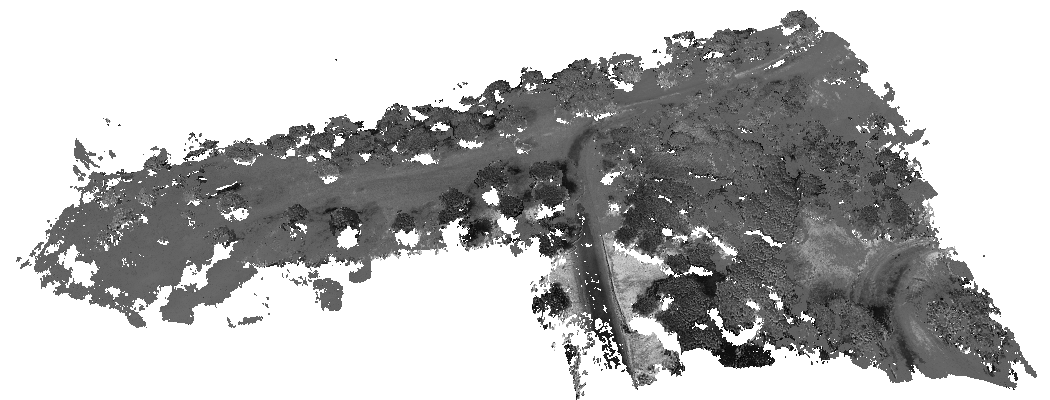
\includegraphics[width=\imageTableSize]{figs/multi_thermal_projection/results/metashape/AgisoftThermalMarmolejo.png}} & \multicolumn{1}{m{\imageTableSize}}{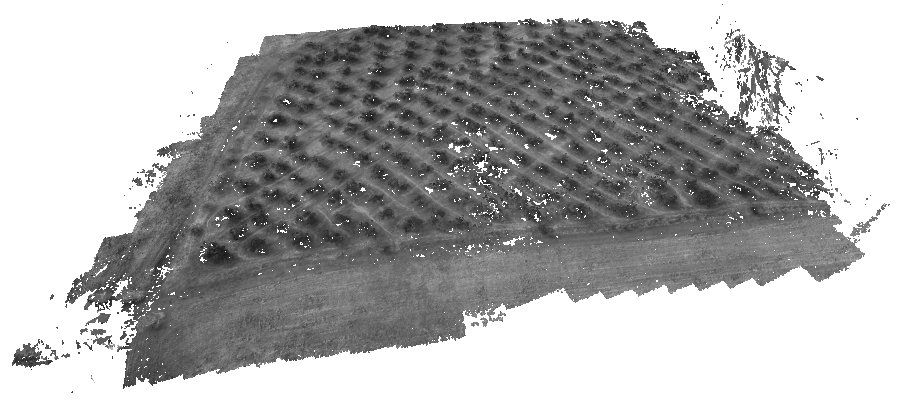
\includegraphics[width=\imageTableSize]{figs/multi_thermal_projection/results/metashape/AgisoftThermalNovember.png}}\\
    & Multispectral & \multicolumn{1}{m{\imageTableSize}|}{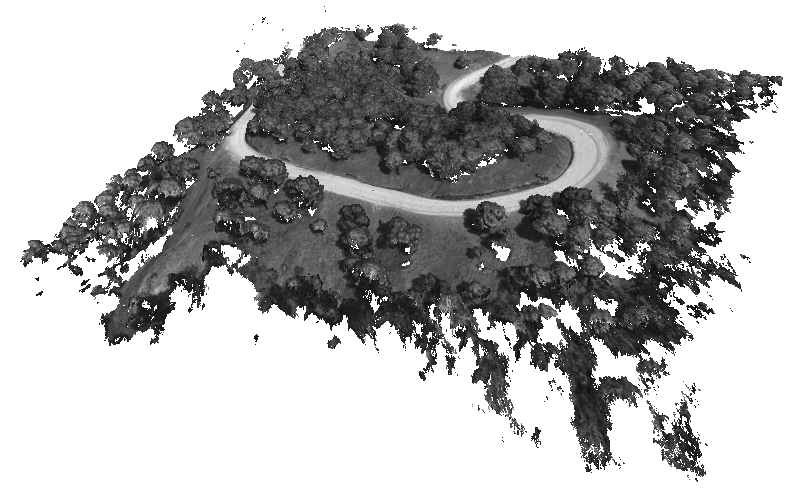
\includegraphics[width=\imageTableSize]{figs/multi_thermal_projection/results/metashape/AgisoftMultispectralMarmolejo.png}} & \multicolumn{1}{m{\imageTableSize}}{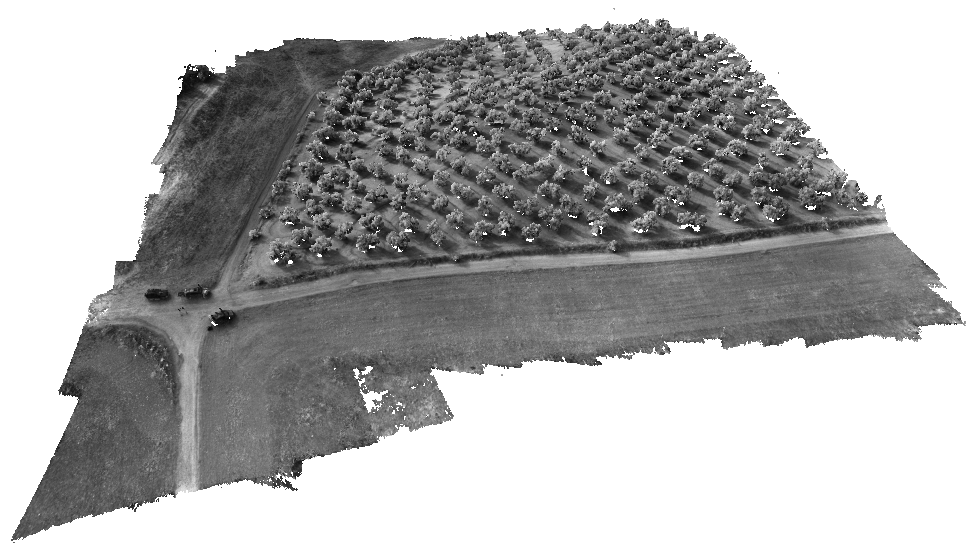
\includegraphics[width=\imageTableSize]{figs/multi_thermal_projection/results/metashape/AgisoftMultispectralNovember.png}}\\
    \cmidrule{1-4}
    \multirow{2}{*}[-4.1em]{Pix4Dmapper} & Thermal & \multicolumn{1}{m{\imageTableSize}|}{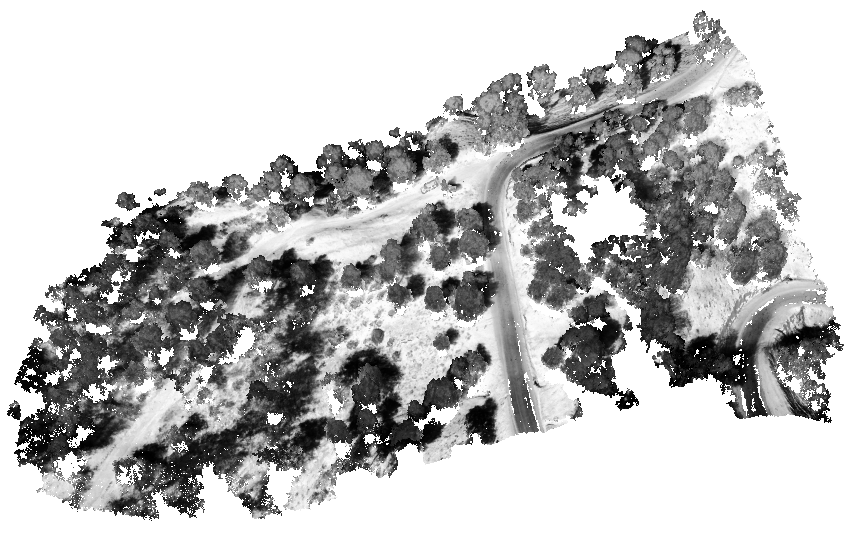
\includegraphics[width=\imageTableSize]{figs/multi_thermal_projection/results/pix4dmapper/Pix4DThermalMarmolejo.png}} & \multicolumn{1}{m{\imageTableSize}}{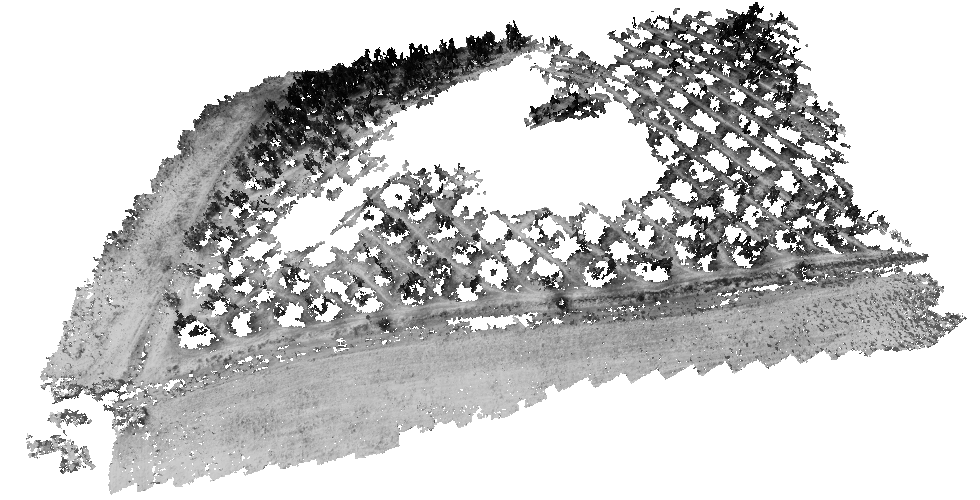
\includegraphics[width=\imageTableSize]{figs/multi_thermal_projection/results/pix4dmapper/Pix4DThermalNovember.png}}\\
    & Multispectral & \multicolumn{1}{m{\imageTableSize}|}{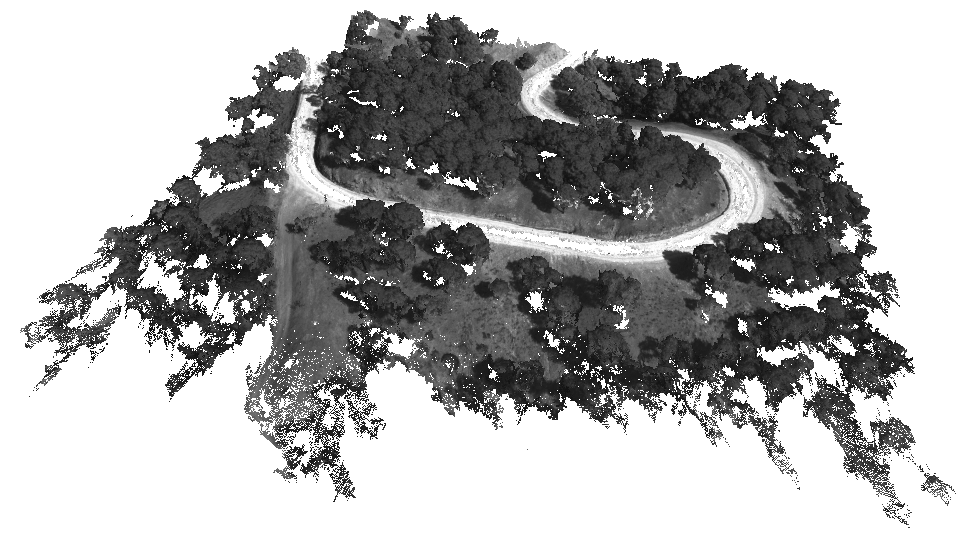
\includegraphics[width=\imageTableSize]{figs/multi_thermal_projection/results/pix4dmapper/Pix4DMultispectralMarmolejo.png}} & \multicolumn{1}{m{\imageTableSize}}{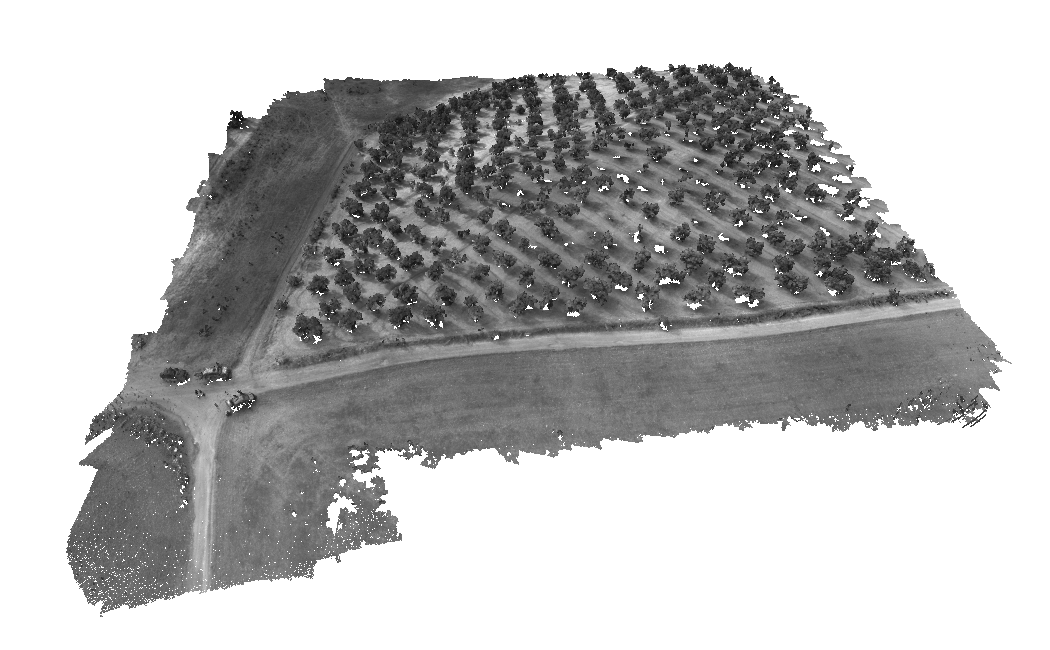
\includegraphics[width=\imageTableSize]{figs/multi_thermal_projection/results/pix4dmapper/Pix4DMultispectralNovember.png}}\\
    \cmidrule{1-4}
    \multirow{2}{*}[-4.1em]{Our method} & Thermal & \multicolumn{1}{m{\imageTableSize}|}{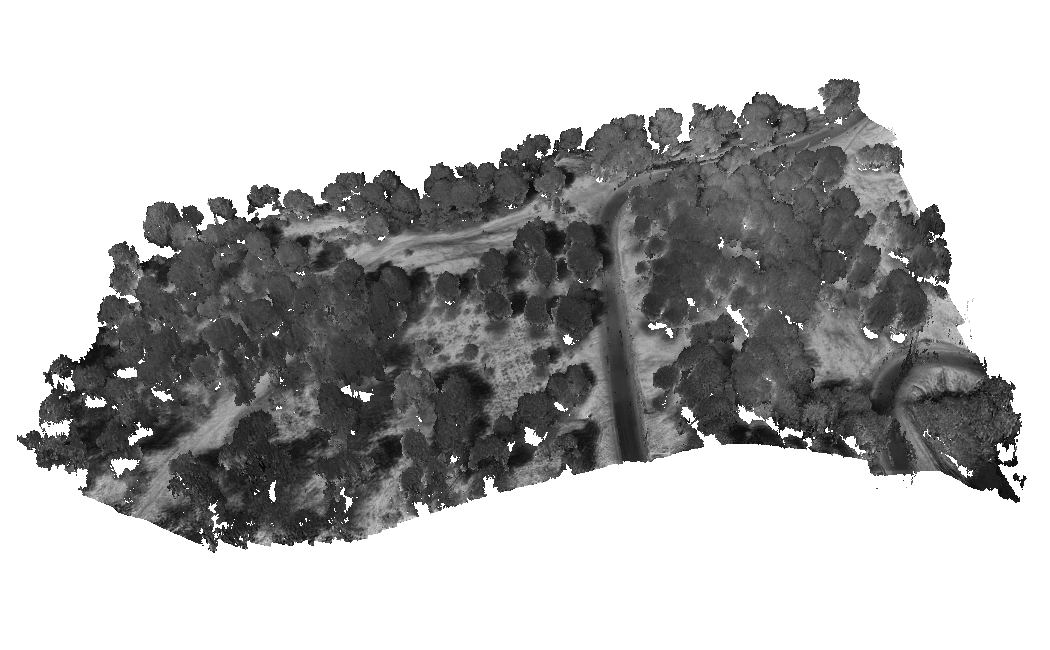
\includegraphics[width=\imageTableSize]{figs/multi_thermal_projection/results/ours/OurThermalMarmolejo.png}} & \multicolumn{1}{m{\imageTableSize}}{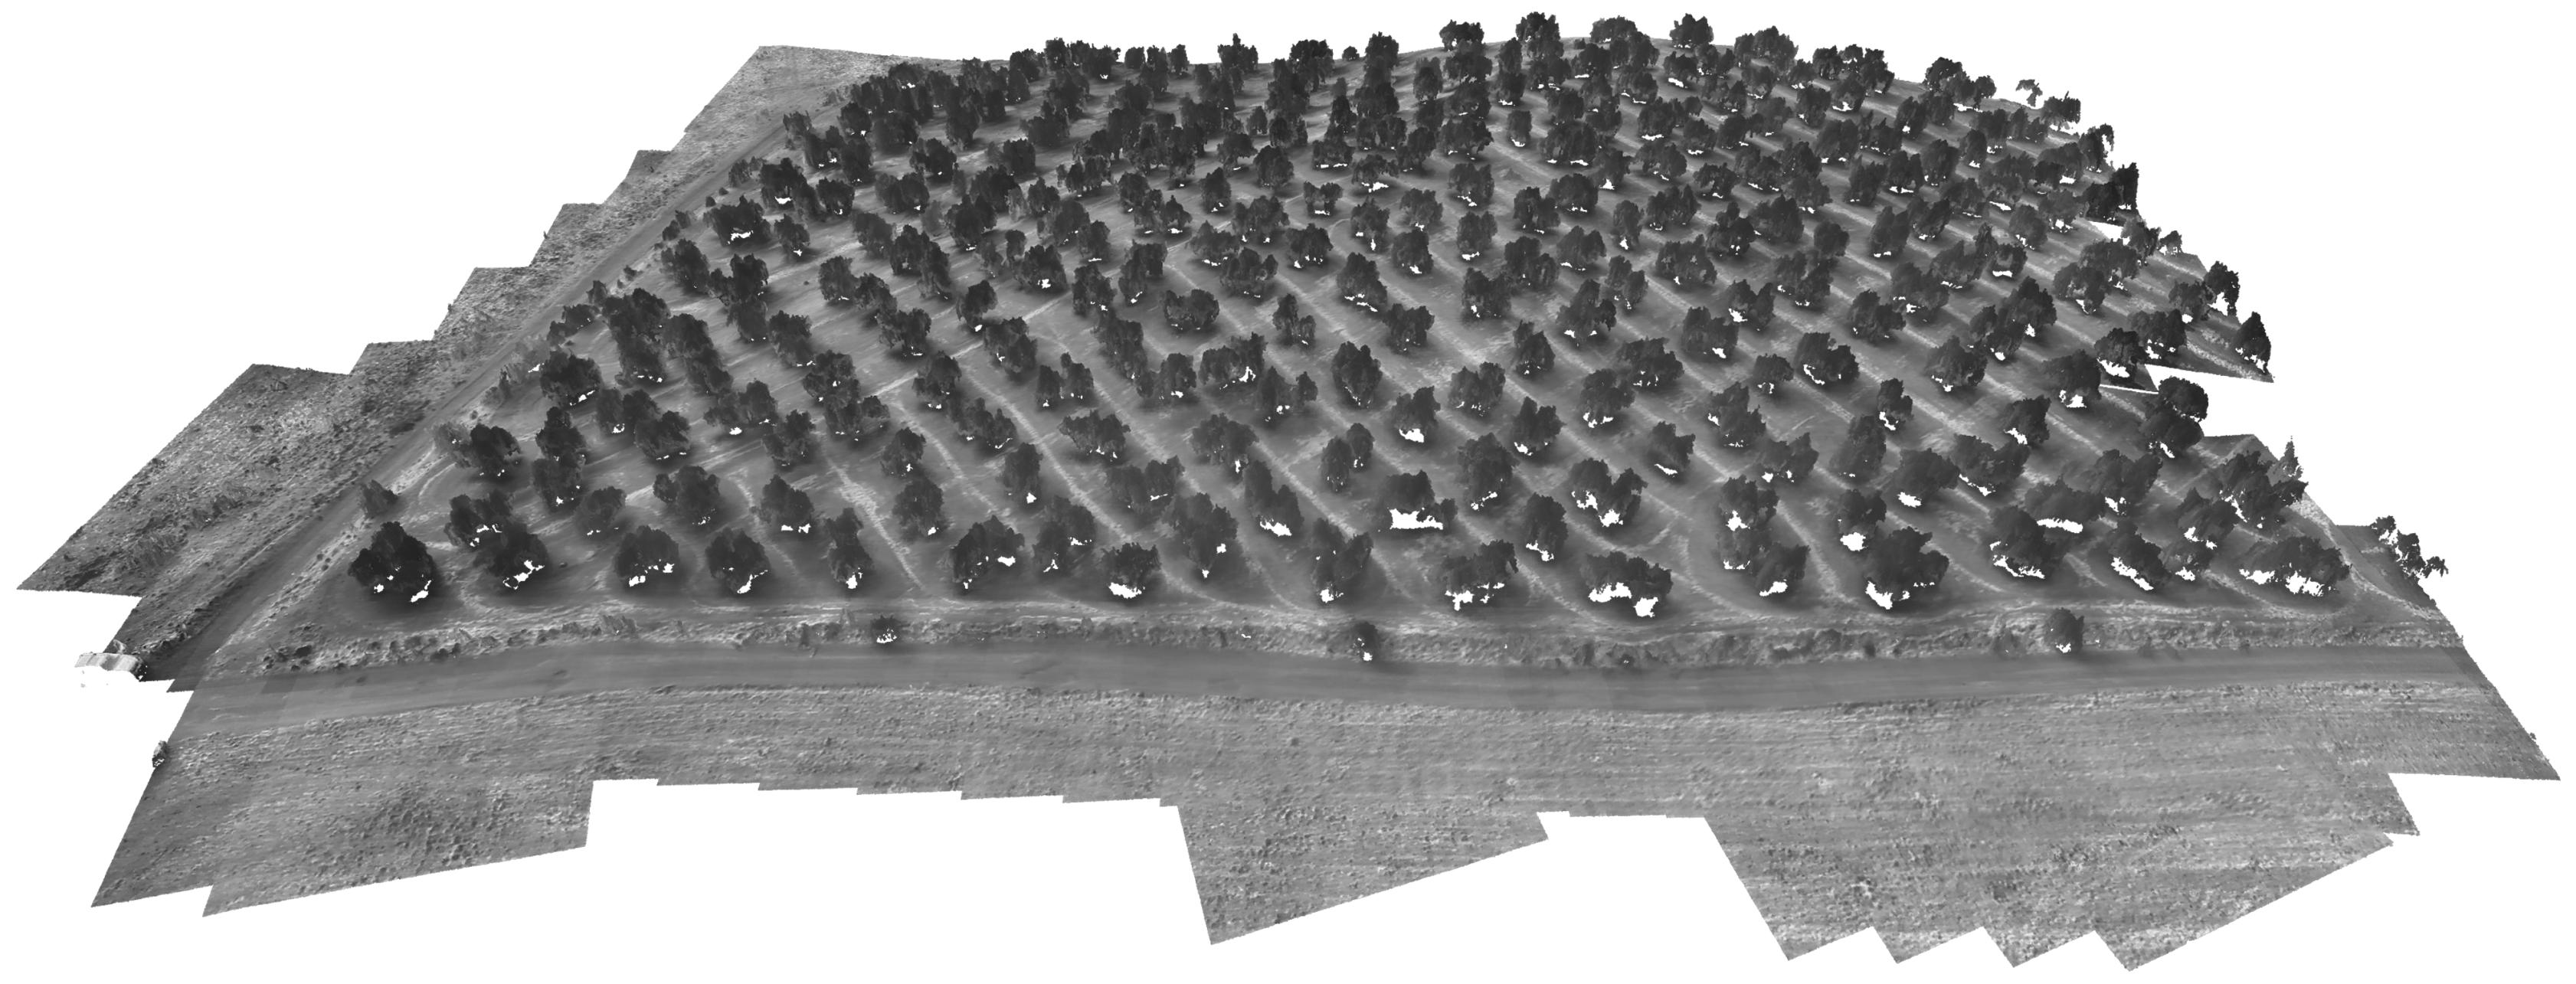
\includegraphics[width=\imageTableSize]{figs/multi_thermal_projection/results/ours/OurThermalNovember2.png}}\\
    & Multispectral & \multicolumn{1}{m{\imageTableSize}|}{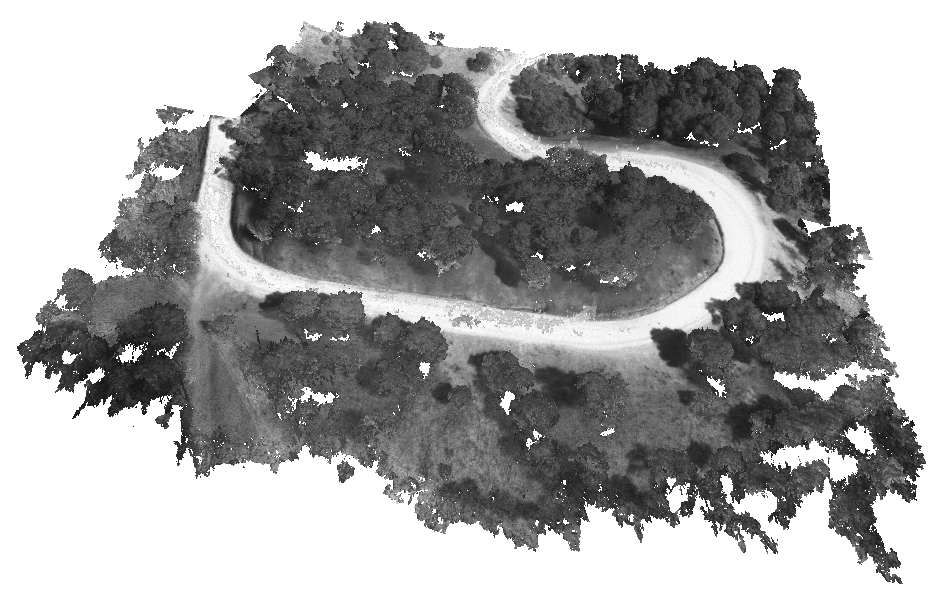
\includegraphics[width=\imageTableSize]{figs/multi_thermal_projection/results/ours/OurMultispectralMarmolejo.png}} & \multicolumn{1}{m{\imageTableSize}}{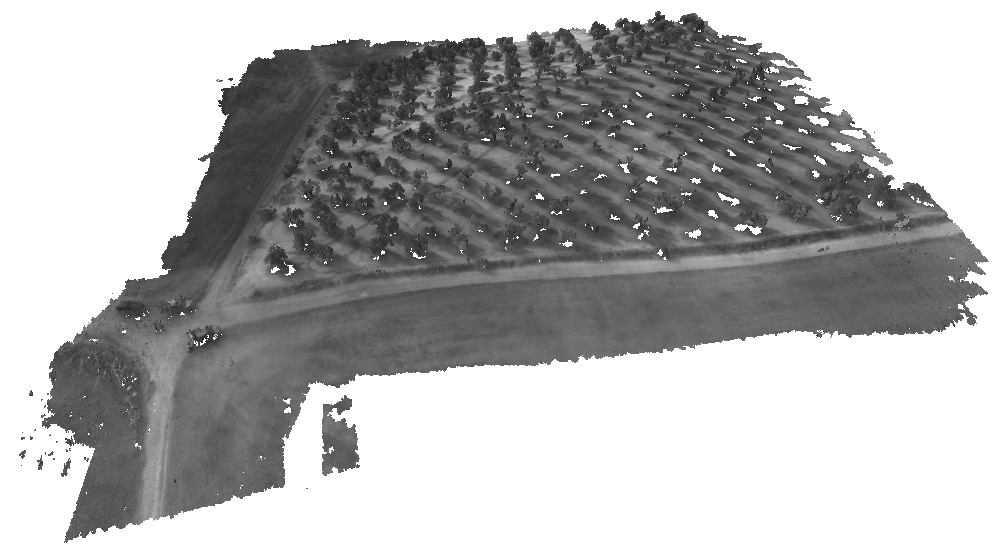
\includegraphics[width=\imageTableSize]{figs/multi_thermal_projection/results/ours/OurMultispectralNovember.png}}\\
    \bottomrule
    \end{tabular}
\end{table*}

